%%%%%%%%%%%%%%%%%%%%%%%%%%%%%%%%%%%%%%%%%
% Short Sectioned Assignment LaTeX Template Version 1.0 (5/5/12)
% This template has been downloaded from: http://www.LaTeXTemplates.com
% Original author:  Frits Wenneker (http://www.howtotex.com)
% License: CC BY-NC-SA 3.0 (http://creativecommons.org/licenses/by-nc-sa/3.0/)
%%%%%%%%%%%%%%%%%%%%%%%%%%%%%%%%%%%%%%%%%

%----------------------------------------------------------------------------------------
%	PACKAGES AND OTHER DOCUMENT CONFIGURATIONS
%----------------------------------------------------------------------------------------

\documentclass[paper=a4, fontsize=11pt]{scrartcl} % A4 paper and 11pt font size

% ---- Entrada y salida de texto -----


\usepackage[dvipsnames]{xcolor}
\usepackage{colortbl}
\usepackage{verbatim}
\usepackage{booktabs}
\usepackage{enumitem}
\newlist{subquestion}{enumerate}{1}
\setlist[subquestion,1]{label=(\alph*)}
\usepackage[T1]{fontenc} % Use 8-bit encoding that has 256 glyphs
\usepackage[utf8]{inputenc}
%\usepackage{fourier} % Use the Adobe Utopia font for the document - comment this line to return to the LaTeX default

% ---- Idioma --------

\usepackage[spanish, es-tabla]{babel} % Selecciona el español para palabras introducidas automáticamente, p.ej. "septiembre" en la fecha y especifica que se use la palabra Tabla en vez de Cuadro

% ---- Otros paquetes ----

\usepackage{url} % ,href} %para incluir URLs e hipervínculos dentro del texto (aunque hay que instalar href)
\usepackage{amsmath,amsfonts,amsthm} % Math packages
%\usepackage{graphics,graphicx, floatrow} %para incluir imágenes y notas en las imágenes
\usepackage{graphics,graphicx, float, subfig} %para incluir imágenes y colocarlas

% Para hacer tablas comlejas
%\usepackage{multirow}
%\usepackage{threeparttable}

%\usepackage{sectsty} % Allows customizing section commands
%\allsectionsfont{\centering \normalfont\scshape} % Make all sections centered, the default font and small caps

\usepackage{fancyhdr} % Custom headers and footers
\pagestyle{fancyplain} % Makes all pages in the document conform to the custom headers and footers
\usepackage{eurosym} % Para poder añadir el símbolo del euro
\fancyhead{} % No page header - if you want one, create it in the same way as the footers below
\fancyfoot[L]{} % Empty left footer
\fancyfoot[C]{} % Empty center footer
\fancyfoot[R]{\thepage} % Page numbering for right footer
\renewcommand{\headrulewidth}{0pt} % Remove header underlines
\renewcommand{\footrulewidth}{0pt} % Remove footer underlines
\setlength{\headheight}{13.6pt} % Customize the height of the header

\numberwithin{equation}{section} % Number equations within sections (i.e. 1.1, 1.2, 2.1, 2.2 instead of 1, 2, 3, 4)
\numberwithin{figure}{section} % Number figures within sections (i.e. 1.1, 1.2, 2.1, 2.2 instead of 1, 2, 3, 4)
\numberwithin{table}{section} % Number tables within sections (i.e. 1.1, 1.2, 2.1, 2.2 instead of 1, 2, 3, 4)

\setlength\parindent{0pt} % Removes all indentation from paragraphs - comment this line for an assignment with lots of text

\newcommand{\horrule}[1]{\rule{\linewidth}{#1}} % Create horizontal rule command with 1 argument of height


\usepackage{algpseudocode}
\usepackage[spanish]{babel}
\usepackage{varwidth}
\usepackage{hyperref}

\selectlanguage{spanish} 
\usepackage[spanish,onelanguage]{algorithm2e} %for psuedo code
\usepackage[lmargin=3.81cm,tmargin=2.54cm,rmargin=2.54cm,bmargin=2.52cm]{geometry}
%\usepackage{listings}
%\usepackage{dsfont}

%----------------------------------------------------------------------------------------
%	TÍTULO Y DATOS DEL ALUMNO
%----------------------------------------------------------------------------------------

\title{	
\normalfont \normalsize 
\textsc{\textbf{Metaheurísticas(2019-2020)} \\ Doble Grado en Ingeniería Informática y Matemáticas \\ Universidad de Granada} \\ [25pt] % Your university, school and/or department name(s)
\horrule{0.5pt} \\[0.4cm] % Thin top horizontal rule
\huge Técnicas de Búsqueda basadas en Poblaciones \\ para el Problema de la Máxima Diversidad  (MDP) \\ % The assignment title
\horrule{2pt} \\[0.5cm] % Thick bottom horizontal rule
}
\author{Alberto Jesús Durán López \\ 
DNI: 54142189-M \\
albduranlopez@gmail.com \\
\hfill \break \hspace{1cm}\\
Grupo Jueves, 17:30 - 19:30 } % Nombre y apellidos


\date{\normalsize\today} % Incluye la fecha actual

%----------------------------------------------------------------------------------------
% DOCUMENTO
%----------------------------------------------------------------------------------------

\begin{document}

\maketitle % Muestra el Título

\newpage %inserta un salto de página

\tableofcontents % para generar el índice de contenidos

% \listoffigures

% \listoftables

\newpage


\section{Introducción}
\hspace{1.5cm} Durante el transcurso de la asignatura trabajaremos con el problema de la máxima diversidad \textit{(Max Diversity Problem)}. 


En particular, en esta práctica estudiaremos técnicas de Búsqueda basadas en Poblaciones para la resolución del problema en cuestión. \\
Comentaremos todos los pasos y problemas encontrados, detallando minuciosamente todos los detalles y solución a los mismos, comenzando con los dos tipos de Algoritmos Genéticos implementados y terminando con Algoritmos Meméticos. \\

Además, se incorporarán tablas para mostrar los resultados de todas las ejecuciones y  gráficas para contrastar los modelos (optimización, costes y desviación).


\section{Problema de la máxima Diversidad}
\hspace{1.5cm} El problema de la máxima diversidad (\textit{maximum diversity problem}, MDP) es un problema de optimización combinatoria consistente en seleccionar un subconjunto de m elementos ($|M|=m$) de un conjunto inicial N de n elementos (con $n>m$) de forma que se maximice la diversidad entre los elementos escogidos. \\


El \textbf{MDP} se puede formular como: \\


\[
\text{Maximizar:   }  z_{MS}(x) = \sum_{i=1}^{n-1} \sum_{j=i+1}^{n} d_{ij}x_i x_j
\]



\[
\text{Sujeto a: } \sum_{i=1}^{n} x_i=m \hspace{0.2cm} \text{ con } x_i=\{0,1\} \text{, } i=1,...,n  \hspace{0.5cm} \text{donde: }
\]


\begin{itemize}
	\item x es una solución al problema que consiste en un vector binario que indica los m elementos seleccionados.
	\item $d_{ij}$ es la distancia existente entre los elementos $i$ y $j$
	
\end{itemize}


\begin{figure}[H]
	\centering
	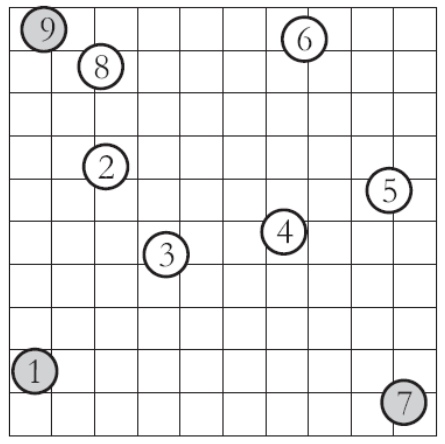
\includegraphics[scale=0.35]{img/mdp.png}
	\caption{MDP-Maximum Diversity Problem}
\end{figure}


\section{Datos y casos considerados}
\hspace{1.5cm} Las ejecuciones se han realizado en un ordenador \texttt{Intel(R) Core(TM) i7-1065G7 CPU @ 1.30GHz, 16GB RAM, 512 SSD}. \\


Se utilizarán \textbf{30 casos} seleccionados de varios de los conjuntos de instancias disponible en la \href{http://www.optsicom.es/mdp/}{MDPLIB}, 10 pertenecientes al grupo \texttt{GKD} con distancias Euclideas, n=500 y m=50 \textit{(GKD-c\_11\_n500\_m50 a GKD-
c\_20\_n500\_m50)}, 10 del grupo \texttt{MDG} con distancias reales en [0,1000], n=500 y m=50
\textit{(MDG-b\_1\_n500\_m50 a MDG-b\_10\_n500\_m50)}; y otras 10 del grupo \texttt{MDG} con distancias enteras en {0,10}, n=2000 y m=200 \textit{(MDG-a\_31\_n2000\_m200 a MDG-
a\_40\_n2000\_m200)}. \\


Para la realización de la práctica usaremos el lenguaje de programación \texttt{C++} ya que se deben probar muchos ejemplos y la ejecución es más rápida al ser un lenguaje de programación compilado. \\
Todos los archivos se han compilado con la opción de optimización \texttt{-O2} y, además,  la semilla usada para todas
las ejecuciones ha sido 54142189, pudiéndose ésta indicar en la ejecución del archivo en cuestión. 






\section{Algoritmos Genéticos}


\subsection{Representación de las Poblaciones}


Para la programación de nuestros Algoritmos Genéticos se han necesitado 2 poblaciones que hemos ido actualizando, la población actual y la población correspondiente a la siguiente generación. Por ello, se ha optado por su encapsulación en una clase que hemos llamado \textit{población}. En ella, se han añadido las variables referentes a la mutación y al cruce, el tamaño de la población o número de cromosomas (que hemos llamado \textbf{n}), el índice del mejor cromosoma de la población (\textbf{best}) y, por último, una matriz de booleanos para representar las distintas soluciones del problema (cada una de tamaño m). \\


\begin{figure}[H]
	\centering
	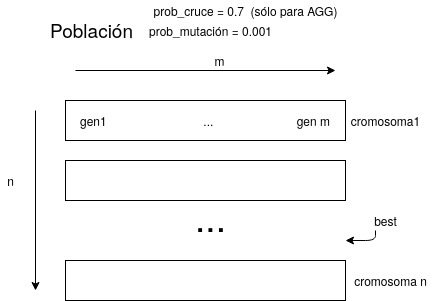
\includegraphics[scale=0.75]{img/a1.jpg}
	\caption{Class poblacion}
\end{figure}


\newpage 
\subsection{Generación de Soluciones Iniciales}
El esquema de la solución inicial varía respecto a la práctica anterior ya que para los Algoritmos Genéticos es necesaria la codificación binaria. Por tanto, cada cromosoma estará formado por valores booleanos 1 (cuando se toma el gen) o 0 (cuando no lo tomamos). Mostramos a continuación el algoritmo para la generación aleatoria de cada cromosoma de nuestra población, teniendo en cuenta que cada uno de los cromosomas debe cumplir las restricciones del problema MDP.

\begin{figure}[H]
	\centering
	\begin{minipage}{.9\linewidth}
		
		
		
		\begin{algorithm}[H] 
			
			\caption{Solución inicial}
			\SetAlgoLined
			
			\KwData{\textbf{Solucion Inicial}$(n_1,m_1)$}
			
			\Begin{
				\textit{vector<bool>}  \textit{cromosoma} \;
				
				\While{\textit{not salir}}{
					
					$cromosoma[random\%n_1] \leftarrow true$ \;
					
					\If{nº de true de cromosoma $= m_1$}{
						$salir \leftarrow true$ \;
					}
				}
				
				\Return $cromosoma$
			}
			
		\end{algorithm} 
		
	\end{minipage}
\end{figure}

$n_1$ y $m_1$ son los índices del problema MDP obtenidos tras leer cada una de las instancias y necesarios para el cumplimiento de las restricciones.



\subsection{Descripción de la Función Objetivo}

Todos los AG implementados hacen uso de la misma función objetivo, la comentada en el punto (2) anterior y cuyo pseudocódigo mostramos a continuación. Bien es cierto que en el caso de los algoritmos meméticos se tiene que pasar a codificación entera, sin embargo, dicha función no se ve modificada.


\begin{figure}[H]
	\centering
	\begin{minipage}{.9\linewidth}
		
		
		
		\begin{algorithm}[H] 
			

			\SetAlgoLined
			
			\KwData{\textbf{ContribucionIndep}(\textit{integer ind, vector sel, matriz distancias)}}
			
			\Begin{
				\textit{suma $\leftarrow$ 0} \;
				
				\For{j in sel}{
					$ suma \leftarrow sel[j]\cdot(distancias[ind][j] + suma)$ \;	
				}
				
				\Return $suma$
			}
			
		\end{algorithm} 
		
	\end{minipage}
\end{figure}



\begin{figure}[H]
	\centering
	\begin{minipage}{.9\linewidth}
		
		
		
		\begin{algorithm}[H] 
			
			\caption{Evaluar solución}
			\SetAlgoLined
			
			\KwData{\textbf{CosteEstimado}(\textit{vector sel, matriz distancias)}}
			
			\Begin{
				
				\textit{suma $\leftarrow$ 0} \;
				
				
				\For{i in $|sel|$}{
					\If{$sel[i]=true$}{
						$ suma \leftarrow ContribucionIndep(i, sel, distancias) + suma$ \;
					}
					
				}
				
				\Return $suma/2$
			}
			
		\end{algorithm} 
		
	\end{minipage}
\end{figure}





\subsection{Esquema de Evolución y de Reemplazamiento}
Se han desarrollado un total de 4 algoritmos genéticos, dos variantes generacionales elitistas (AGG) y otras dos variantes estacionarias(AGE):

\begin{itemize}
	\item \textbf{AGG}: En los Algoritmos Genéticos Generacionales se selecciona una población de padres del mismo tamaño que la población genética usando el operador de Selección, donde cruzaremos los distintos cromosomas mediantes torneos binarios.	
	
	
	
	Por otro lado, están caracterizados por su esquema elitista, es decir, en cada generación se mantiene el mejor elemento de la población. 
	
	
	\begin{figure}[H]
		\centering
		\begin{minipage}{.86\linewidth}
			
			
			
			\begin{algorithm}[H] 
				
				\caption{Operador de Reemplazamiento para AGG}
				\SetAlgoLined
				
				\KwData{\textbf{ReemplazamientoAGG}}
				
				\Begin{
					\If{$poblacion_{antigua}[best] \not \in poblacion_{nueva}$}{
						$poblacion_{nueva}[peor] \leftarrow poblacion_{antigua}[best]$ \;
						
						
					}
					
				}
				
			\end{algorithm} 
			
		\end{minipage}
	\end{figure}
	
	
	\item \textbf{AGE}: Se caracterizan por tener un esquema de evolución donde únicamente se seleccionan dos padres que compiten con los 2 peores de la población. 
	
	
	Los dos descendientes generados tras el cruce y la mutación sustituyen a los dos peores de la población actual (en caso de ser mejores que ellos), tal y como se muestra a continuación:
	
	\begin{figure}[H]
		\centering
		\begin{minipage}{.86\linewidth}
			
			
			
			\begin{algorithm}[H] 
				
				\caption{Operador de Reemplazamiento para AGE}
				\SetAlgoLined
				
				\KwData{\textbf{ReemplazamientoAGE}}
				
				\Begin{
					$peor_1 \leftarrow min\_element(poblacion)$ \;
					
					$peor_2 \leftarrow next\_min\_element(poblacion)$ \;
					
					\If{Coste $descendiente_1 > peor_1$}{
						\textit{Intercambiarlos} \;
					}
					\If{Coste $descendiente_2 > peor_2$}{
						\textit{Intercambiarlos} \;
					}
					
				}
				
			\end{algorithm} 
			
		\end{minipage}
	\end{figure}

\end{itemize}















Por orden de llamada, los distintos operadores son: \textit{Selección, Cruce, Mutación y Reemplazamiento}.

Tanto para los AGG como AGE se han desarrollado dos variantes: una con un cruce basado en posición y otro uniforme.
Las 4 versiones implementadas comparten estos operadores, sin embargo, comentaremos todos los detalles en las siguientes secciones.



\newpage 
\subsubsection{Operador de Selección AGG}

Comenzamos comentando el operador de Selección de los AGG, caracterizado por realizar tantos torneos binarios como individuos existan en la población genética. Para ello, generamos índices aleatorios referentes a distintos cromosomas y los hacemos competir llamando a la función \textbf{Torneo Binario}. Posteriormente, se va añadiendo el ganador de cada torneo a una nueva población.

\begin{figure}[H]
	\centering
	\begin{minipage}{.9\linewidth}
		
		
		
		\begin{algorithm}[H] 
			\SetAlgoLined
			
			\KwData{\textbf{Torneo Binario}(int r, int s)}
			
			
			\hspace{0.7cm} \Return $coste[r]>coste[s]$ ? r : s \;
			
			
		\end{algorithm} 
		
	\end{minipage}
\end{figure}










\begin{figure}[H]
	\centering
	\begin{minipage}{.9\linewidth}
		
		
		
		\begin{algorithm}[H] 
			
			\caption{Operador de Selección}
			\SetAlgoLined
			
			\KwData{\textbf{Seleccion}}
			
			\Begin{
				$poblacion$ $nueva$ \;		
				
				\For{\textit{i in }$|poblacion|$}{
					
					$ganador \leftarrow$ \textbf{TorneoBinario}\textit{(rand,rand)}\;
					$cromosoma \leftarrow poblacion[ganador]$ \;
					$nueva \leftarrow nueva \cup cromosoma$ \;
				}
				
				\Return $nueva$
			}
			
		\end{algorithm} 
		
	\end{minipage}
\end{figure}







\subsection{Operador de Selección AGE}
En este operador, en vez de realizar tantos torneos binarios como individuos haya en la población, se aplicará únicamente 2 veces para elegir los dos padres que posteriormente serán cruzados. Hacemos uso de la función Torneo Binario y devolvemos la pareja de padres obtenidos:

\begin{figure}[H]
	\centering
	\begin{minipage}{.9\linewidth}
		
		
		
		\begin{algorithm}[H] 
			\SetAlgoLined
			
			\KwData{\textbf{Torneo Binario}(int r, int s)}
			
			
			\Return $coste[r]>coste[s]$ ? r : s \;
			
			
		\end{algorithm} 
		
	\end{minipage}
\end{figure}










\begin{figure}[H]
	\centering
	\begin{minipage}{.9\linewidth}
		
		
		
		\begin{algorithm}[H] 
			
			\caption{Operador de Selección}
			\SetAlgoLined
			
			\KwData{\textbf{Seleccion}}
			
			\Begin{
				pair padres \;		
				
				\textbf{hacer}\{ \break
					\text{      }padres.first $\leftarrow$ \textbf{TorneoBinario}\textit{(rand,rand)} \;
					\hspace{0.3cm}padres.second $\leftarrow$ \textbf{TorneoBinario}\textit{(rand,rand)} \;
				\}\textbf{mientras} \textit{padres.first $=$ padres.second}
				
				
				\Return $padres$
			}
			
		\end{algorithm} 
		
	\end{minipage}
\end{figure}




\newpage 

\subsection{Operador de Cruce Posicional}

En este Operador tenemos una probabilidad de cruce de 0.7, por ello, hemos decidido implementar dos versiones. 

\begin{itemize}
	\item La primera, mediante una función que simula una distribución uniforme, generamos un número aleatorio para cada pareja y las cruzamos con probabilidad 0.7
	
	\item En la segunda, estimamos a priori el número de cruces haciendo uso de la \textit{Esperanza Matemática}, donde dicho valor se calculará como  $prob\_cruce \cdot |poblacion|$. Los cromosomas a cruzar serán obtenidos de forma aleatoria.
	
	En ambas versiones el cruce se realiza siempre por parejas consecutivas, el 1º con el 2º, el 3º con el 4º, tal y como se ha descrito en el Seminario 3.
\end{itemize}


Se han hecho pruebas con ambas versiones y se han obtenido unos ligeros mejores resultados en la primera versión ya que forzamos el recorrido de todos los cromosomas y no dependemos de la aleatoriedad en su elección, sin embargo perdemos eficiencia, ya que no hacemos uso de la \textit{Esperanza Matemática}.  Mostramos por ello el pseudocódigo asociado a la segunda versión: (la implementación de ambas versiones está íntegra en el proyecto entregado). 




\begin{figure}[H]
	\centering
	\begin{minipage}{.9\linewidth}
		
		
		
		\begin{algorithm}[H] 
			
			\caption{Cruce Posicional}
			\SetAlgoLined
			
			\KwData{\textbf{Cruce Posicional}}
			
			\Begin{
				\textit{cruces} $\leftarrow prob_{cruce}\cdot N/2$
				
				\While{$cruces>0$}{
					
					\textit{elegir pareja (i, i+1) para cruzarlos}
					$padre_{restos} \leftarrow random(Padre_i, Padre_{i+1})$ \; 
					
					\For{\textit{j in} $|padre_i|$}{
						\If{$Padre_i[j]  = Padre_{i+1}[j]$}{
							$hijo_1[j] \leftarrow padre_i[j]$  \;
							$hijo_2[j] \leftarrow padre_i[j]$
						}
						\Else{
							$restos \leftarrow restos \cup padre_{restos}[j]$ \;
						}
					}
											
					\textit{rellenar aleat. hijo1 con $restos$} \;
					\textit{rellenar aleat. hijo2 con $restos$} \;
					
					\textit{cruces - -} \;
			
				}
			
			}
			
			
		\end{algorithm} 
		
	\end{minipage}
\end{figure}

Destacamos que en cada cruce elegimos un padre aleatorio para después rellenar las posiciones de ambos hijos de forma aleatoria.
En este operador se generan hijos factibles si los dos padres son factibles luego no se necesita reparar las soluciones. Sin embargo, es más disruptivo, comparte menos información de los padres y la convergencia puede ser más costosa.

\newpage 

\subsection{Operador de cruce Uniforme}
En el cruce Uniforme no tenemos el problema descrito anteriormente ya que la probabilidad de cruce es de 1, es decir, siempre se cruzan los dos padres. Sin embargo, este operador requiere reparador ya que las soluciones obtenidas pueden no ser factibles. Cruzamos siempre parejas de cromosomas consecutivas, el 1º con el 2º, 3º con el 4º ...etc. El reparador aplicado es el descrito en las diapositivas del Seminario 3.


Hay que tener en cuenta las siguientes consideraciones:
\begin{itemize}
	\item Por motivos de eficiencia y para no generar un exceso de números aleatorios, cruzamos parejas de cromosomas consecutivas.
	
	\item Las dos variantes de nuestros Algoritmos Genéticos hacen uso de este cruce. En el caso de los AGG, se realiza un cruce uniforme por parejas de toda la población, mientras que en los AGE únicamente se cruzan dos padres. El cruce que mostramos es el que se realiza en los AGG, para los AGE se realiza el mismo cruce pero únicamente para la pareja que se cruza, no para toda la población.
\end{itemize}

\begin{figure}[H]
	\centering
	\begin{minipage}{.9\linewidth}
		
		
		
		\begin{algorithm}[H] 
			
			\caption{Cruce Uniforme}
			\SetAlgoLined
			
			\KwData{\textbf{Cruce Uniforme}\textit{(integer m)}}
			
			\Begin{
				
				\textit{cruces} $\leftarrow prob_{cruce}\cdot N/2$ \;
				
				\While{cruces>0}{
					
					\textit{Elegir pareja de Cromosomas $(i,i+1)$} \;
				
					$padre_r=random(padre_i, padre_{i+1})$ \;
					$padre_s=random(padre_i, padre_{i+1})$ \;
					
					\For{\textit{j in} $|padre_i|$}{
						\If{$Padre_i[j] = Padre_{i+1}[j]$}{
							$hijo_1[j] \leftarrow padre_i[j]$  \;
							$hijo_2[j] \leftarrow padre_i[j]$
						}
						\Else{
							//Rellenamos los hijos con los restos de un padre aleat. \;
							$hijo_1[j] \leftarrow padre_r[j]$ \;
							$hijo_2[j] \leftarrow padre_s[j]$ \;
						}
				}
						
				\textbf{reparar}\textit{($hijo_1$,m)}\;
				\textbf{reparar}\textit{($hijo_2$,m)}\;
					
				\textit{cruces - -} \;
					
				
				}
			}
			
		\end{algorithm} 
		
	\end{minipage}
\end{figure}

Recorremos ambos padres. En aquellas posiciones que contengan el mismo valor en ambos padres se mantienen en el hijo para así preservar las selecciones prometedores.
En otro caso, las selecciones restantes serán rellenadas por los valores de uno de los padres.














\newpage 
\subsection{Operador de Mutación}
Para el operador de mutación consideramos una probabilidad de mutación por gen de 0.001. Para que nuestro problema siga cumpliendo las restricciones, intercambiaremos un gen $x_i$ por otro $x_j$ dentro de un mismo cromosoma/solución de nuestra población, comprobando que los valores a intercambiar sean opuestos, es decir, un 0 por un 1. Por tanto, las soluciones seguirán siendo factibles y no será necesaria ninguna comprobación ni reparación posterior. \\



Al igual que ocurre en el operador de cruce, uno de los problemas más costosos y más ineficientes de los algoritmos genéticos es la generación de números aleatorios. Como en este operador este problema está intensificado (ya que la prob\_cruce es de 0.001), volvemos a diseñar una implementación basada en la \textit{Esperanza Matemática} para así reducir en gran medida la cantidad de números aleatorios generados y, como consecuencia, reducir el tiempo de ejecución lo máximo posible.  \\


El pseudocódigo correspondiente a dicho operador es el siguiente: 


\begin{figure}[H]
	\centering
	\begin{minipage}{.9\linewidth}
		
		
		
		\begin{algorithm}[H] 
			
			
			
			\caption{Operador de Mutación}
			\SetAlgoLined
			
			\KwData{\textbf{Mutacion}}
			
			\Begin{
				total $\leftarrow$ $prob\_mut\cdot nºgenes$ $total$\;
				\textit{suma $\leftarrow$ 0} \;
				
				
				\While{$total>0$}{
					 $n_1 \leftarrow$ \textit{índice para elegir cromosoma} \;
					 $m_1 \leftarrow$ \textit{índice para elegir gen} \;
					
					\textbf{hacer} \{  \break
					\hspace{1cm}$m_2 \leftarrow$ \textit{índice para elegir gen distinto a $m_1$} \;
					\} \textbf{mientras}(\textit{los dos genes sean iguales}) \;
					
					\textit{Intercambiar genes} \;
					
					\textit{total - -} \;
					
				}
				
			}
			
		\end{algorithm} 
		
	\end{minipage}
\end{figure}


Generamos 3 números aleatorios. El primero $n_1$ para elegir el cromosoma y, los dos posteriores $m_1$ y $m_2$, para intercambiar dos genes dentro de éste. Para el intercambio de los genes comprobamos que sean del mismo cromosoma (para no violar las restricciones) y que dichos genes sean distintos (uno cero y el otro uno), como hemos comentado anteriormente.

El pseudocódigo anterior es el de los AGG ya que involucra a toda la población de cromosomas. El referente a AGE es una pequeña variante del anterior en el que únicamente se toman los dos padres.





\newpage 
\section{Algoritmos Meméticos}

\hspace{1.5cm} Nuestro Algoritmo Memético consistirá en una técnica de hibridación de un Algoritmo Genético Generacional con una BL (la desarrollada en la práctica 1).

Nuestro problema MDP se complica ya que para aplicar la búsqueda local es necesario pasar de codificación binaria a codificación de conjuntos enteros, sin embargo, esto no supone ninguna modificación en el resto de funciones implementadas. \\

Se han realizado tres posibilidades de hibridación, combinando y manteniendo un equilibrio distinto entre exploración y explotación.
Adelantamos que en todas ellas se usa la estrategia con el operador de cruce basado en posición ya que se han obtenido mejores resultados que con el uniforme. \\

El tamaño de la población del AGG cambia y pasará a tener 10 cromosomas. Sin embargo, las probabilidades de cruce y mutación se mantienen a 0.7 y 0.001, respectivamente.



Por otro lado, la búsqueda local se detendrá cuando realice 400 evaluaciones de vecinos distintos o no encuentre mejora en el entorno.
El criterio de parada del AM consistirá en realizar 100.000 evaluaciones de la función objetivo, incluyendo además las de la BL.

\begin{itemize}
	\item \texttt{AM-(10,1.0)}:	Cada \textbf{10} generaciones aplicaremos Búsqueda Local sobre \textbf{todos los cromosomas} de la población. Predomina la exploración sobre la explotación, ya que la BL consume las evaluaciones muy rápido, sin embargo, no se deja a ningún cromosoma atrás y favorece la diversidad de las soluciones.
	\item \texttt{AM-(10,0.1)}:	Cada \textbf{10} generaciones aplicaremos la Búsqueda Local sobre un \textbf{subconjunto de cromosomas} de la población seleccionando aleatoriamente con probabilidad de \textbf{0.1} para cada uno de ellos. Tando la exploración como la explotación predominan por igual.
	\item \texttt{AM-(10,0.1mej)}: Cada \textbf{10} generaciones aplicaremos Búsqueda Local sobre los \textbf{0.1}$\cdot$ \textbf{N mejores} cromosomas de la población actual. (N es el tamaño de ésta). Predomina más la explotación que la exploración, se busca a toda costa mejorar el resultado de la función objetivo aplicando BL sobre los cromosomas más prometedores, dejando atrás los que peores resultados arrojan.
\end{itemize}


Las tres variantes se han implementado en un mismo archivo \texttt{.cpp}. Se ha usado la estructura de control \texttt{switch} que ejecutará una u otra según el valor de la variable \texttt{tipo}. Como en nuestros algoritmos se ha optado por la encapsulación de la población en una clase, dicha variable se podrá modificar en el constructor de la misma. 

\newpage 
Mostramos el pseudocódigo asociado a estas tres variantes:
\begin{figure}[H]
	\centering
	\begin{minipage}{.9\linewidth}
		
		
		
		\begin{algorithm}[H] 
			
			\caption{Algoritmos Meméticos}
			\SetAlgoLined
			
			\KwData{\textbf{Algoritmos Meméticos}}
			
			\Begin{
				\textit{Pasar Población a Codificación Entera} \;
				
				\textbf{switch} \textit{(tipo)} \break
				\text{ } \textbf{case} \texttt{ AM-(10,1.0):} \break 
				\text{  } \hspace{0.3cm} \textbf{para} \textit{i in $|poblacion|$} \break
				\text{  } \hspace{0.8cm} $cromosoma$ $\leftarrow$ $poblacion[i]$ \;
				\text{  } \hspace{1cm} $poblacion[i]$ $\leftarrow$ \textbf{BusquedaLocal}\textit{($cromosoma$ , eval)}\;
				\text{  } \hspace{0.4cm}
				\text{} \textbf{break} \;
				
				
				
				\hfill \break 
				\text{ } \textbf{case} \texttt{ AM-(10,0.1):} \break 
				\text{  } \hspace{0.3cm} $total \leftarrow prob\_ls \cdot n$ \;
				\text{  } \hspace{0.5cm} \textbf{mientras} $total>0$ \{ \break
				\text{  } \hspace{0.85cm} $r \leftarrow rand()\%n$ \;
				\text{  } \hspace{1cm} $cromosoma$ $\leftarrow$ $poblacion[r]$ \;
				
				\text{  } \hspace{1cm} $poblacion[r]$ $\leftarrow$ \textbf{BusquedaLocal}\textit{($cromosoma$ , eval)}\;
				\text{  } \hspace{1cm} \textit{total - -} \;
				\text{  } \hspace{0.45cm} \} \break
				\text{} \hspace{0.4cm} \textbf{break} \;
				
				
				
				\hfill \break 
				\text{ } \textbf{case} \texttt{ AM-(10,0.1mej):} \break 
				\text{  } \hspace{0.3cm} $n\_mejores \leftarrow prob\_ls \cdot n$ \;
				\text{  } \hspace{0.5cm} $aux \leftarrow$ \textit{Índices de los n\_mejores cromosomas}\; \break
				\text{  } \hspace{0.5cm} \textbf{para} \textit{i in $aux$} \textbf{hacer}\{ \break
				\text{  } \hspace{0.8cm} $cromosoma$ $\leftarrow$ $poblacion[i]$ \;
				\text{  } \hspace{1cm} $poblacion[i]$ $\leftarrow$ \textbf{BusquedaLocal}\textit{($cromosoma$ , eval)}\;
				\text{  } \hspace{0.5cm} \} \break
				\text{} \hspace{0.4cm} \textbf{break} \;
				
				
				
				
				
								
				

				\textit{Pasar Población a Codificación Binaria} \;
				
				
			}
			
		\end{algorithm} 
		
	\end{minipage}
\end{figure}







\newpage
\section{Resultados}

\subsection{Algoritmos Genéticos Generacionales}




% Please add the following required packages to your document preamble:
% \usepackage{booktabs}
% \usepackage{graphicx}
% \usepackage[table,xcdraw]{xcolor}
% If you use beamer only pass "xcolor=table" option, i.e. \documentclass[xcolor=table]{beamer}
\begin{table}[H]
	\centering
	\resizebox{\textwidth}{!}{%
		\begin{tabular}{@{}
				>{\columncolor[HTML]{FFFFFF}}c 
				>{\columncolor[HTML]{FFFFFF}}c 
				>{\columncolor[HTML]{FFFFFF}}c 
				>{\columncolor[HTML]{FFFFFF}}c 
				>{\columncolor[HTML]{FFFFFF}}c 
				>{\columncolor[HTML]{FFFFFF}}c 
				>{\columncolor[HTML]{FFFFFF}}c 
				>{\columncolor[HTML]{FFFFFF}}c @{}}
			\toprule
			{\color[HTML]{000000} \textbf{Instancia}}     & {\color[HTML]{000000} \textbf{Mejor coste}} & {\color[HTML]{000000} \textbf{AGGp}} & {\color[HTML]{000000} \textbf{Desv}} & {\color[HTML]{000000} \textbf{Time}} & \textbf{AGGu}                  & \textbf{Desv}               & \textbf{Time}                 \\ \midrule
			{\color[HTML]{000000} GKD-c\_11\_n500\_m50}   & {\color[HTML]{000000} 19587,13}             & {\color[HTML]{000000} 19586,2}       & {\color[HTML]{000000} 0,00}          & {\color[HTML]{000000} 16,91}         & {\color[HTML]{000000} 19561,4} & {\color[HTML]{000000} 0,13} & {\color[HTML]{000000} 69,98}  \\
			{\color[HTML]{000000} GKD-c\_12\_n500\_m50}   & {\color[HTML]{000000} 19360,23}             & {\color[HTML]{000000} 19359,6}       & {\color[HTML]{000000} 0,00}          & {\color[HTML]{000000} 16,05}         & {\color[HTML]{000000} 19352,3} & {\color[HTML]{000000} 0,04} & {\color[HTML]{000000} 76,26}  \\
			{\color[HTML]{000000} GKD-c\_13\_n500\_m50}   & {\color[HTML]{000000} 19366,69}             & {\color[HTML]{000000} 19361,0}       & {\color[HTML]{000000} 0,03}          & {\color[HTML]{000000} 15,91}         & {\color[HTML]{000000} 19361}   & {\color[HTML]{000000} 0,03} & {\color[HTML]{000000} 78,76}  \\
			{\color[HTML]{000000} GKD-c\_14\_n500\_m50}   & {\color[HTML]{000000} 19458,56}             & {\color[HTML]{000000} 19458,2}       & {\color[HTML]{000000} 0,00}          & {\color[HTML]{000000} 16,30}         & {\color[HTML]{000000} 19445,5} & {\color[HTML]{000000} 0,07} & {\color[HTML]{000000} 80,16}  \\
			{\color[HTML]{000000} GKD-c\_15\_n500\_m50}   & {\color[HTML]{000000} 19422,15}             & {\color[HTML]{000000} 19422,1}       & {\color[HTML]{000000} 0,00}          & {\color[HTML]{000000} 16,00}         & {\color[HTML]{000000} 19412,7} & {\color[HTML]{000000} 0,05} & {\color[HTML]{000000} 80,44}  \\
			{\color[HTML]{000000} GKD-c\_16\_n500\_m50}   & {\color[HTML]{000000} 19680,20}             & {\color[HTML]{000000} 19679,5}       & {\color[HTML]{000000} 0,00}          & {\color[HTML]{000000} 16,27}         & {\color[HTML]{000000} 19668,1} & {\color[HTML]{000000} 0,06} & {\color[HTML]{000000} 75,37}  \\
			{\color[HTML]{000000} GKD-c\_17\_n500\_m50}   & {\color[HTML]{000000} 19331,38}             & {\color[HTML]{000000} 19331,4}       & {\color[HTML]{000000} 0,00}          & {\color[HTML]{000000} 16,06}         & {\color[HTML]{000000} 19325,1} & {\color[HTML]{000000} 0,03} & {\color[HTML]{000000} 79,72}  \\
			{\color[HTML]{000000} GKD-c\_18\_n500\_m50}   & {\color[HTML]{000000} 19461,39}             & {\color[HTML]{000000} 19460}         & {\color[HTML]{000000} 0,01}          & {\color[HTML]{000000} 16,18}         & {\color[HTML]{000000} 19446,7} & {\color[HTML]{000000} 0,08} & {\color[HTML]{000000} 73,45}  \\
			{\color[HTML]{000000} GKD-c\_19\_n500\_m50}   & {\color[HTML]{000000} 19477,32}             & {\color[HTML]{000000} 19477,3}       & {\color[HTML]{000000} 0,00}          & {\color[HTML]{000000} 16,01}         & {\color[HTML]{000000} 19464,4} & {\color[HTML]{000000} 0,07} & {\color[HTML]{000000} 72,37}  \\
			{\color[HTML]{000000} GKD-c\_20\_n500\_m50}   & {\color[HTML]{000000} 19604,84}             & {\color[HTML]{000000} 19604,8}       & {\color[HTML]{000000} 0,00}          & {\color[HTML]{000000} 15,65}         & {\color[HTML]{000000} 19588,4} & {\color[HTML]{000000} 0,08} & {\color[HTML]{000000} 72,15}  \\
			{\color[HTML]{000000} MDG-b\_1\_n500\_m50}    & {\color[HTML]{000000} 778030,62}            & {\color[HTML]{000000} 755790}        & {\color[HTML]{000000} 2,86}          & {\color[HTML]{000000} 15,86}         & {\color[HTML]{000000} 760558}  & {\color[HTML]{000000} 2,25} & {\color[HTML]{000000} 71,94}  \\
			{\color[HTML]{000000} MDG-b\_2\_n500\_m50}    & {\color[HTML]{000000} 779963,68}            & {\color[HTML]{000000} 762735}        & {\color[HTML]{000000} 2,21}          & {\color[HTML]{000000} 16,15}         & {\color[HTML]{000000} 756991}  & {\color[HTML]{000000} 2,95} & {\color[HTML]{000000} 72,62}  \\
			{\color[HTML]{000000} MDG-b\_3\_n500\_m50}    & {\color[HTML]{000000} 776768,43}            & {\color[HTML]{000000} 759655}        & {\color[HTML]{000000} 2,20}          & {\color[HTML]{000000} 16,07}         & {\color[HTML]{000000} 767226}  & {\color[HTML]{000000} 1,23} & {\color[HTML]{000000} 72,32}  \\
			{\color[HTML]{000000} MDG-b\_4\_n500\_m50}    & {\color[HTML]{000000} 775394,62}            & {\color[HTML]{000000} 752398}        & {\color[HTML]{000000} 2,97}          & {\color[HTML]{000000} 16,69}         & {\color[HTML]{000000} 746584}  & {\color[HTML]{000000} 3,72} & {\color[HTML]{000000} 72,93}  \\
			{\color[HTML]{000000} MDG-b\_5\_n500\_m50}    & {\color[HTML]{000000} 775611,06}            & {\color[HTML]{000000} 759879}        & {\color[HTML]{000000} 2,03}          & {\color[HTML]{000000} 19,11}         & {\color[HTML]{000000} 750147}  & {\color[HTML]{000000} 3,28} & {\color[HTML]{000000} 79,06}  \\
			{\color[HTML]{000000} MDG-b\_6\_n500\_m50}    & {\color[HTML]{000000} 775153,68}            & {\color[HTML]{000000} 758308}        & {\color[HTML]{000000} 2,17}          & {\color[HTML]{000000} 17,87}         & {\color[HTML]{000000} 748763}  & {\color[HTML]{000000} 3,40} & {\color[HTML]{000000} 77,12}  \\
			{\color[HTML]{000000} MDG-b\_7\_n500\_m50}    & {\color[HTML]{000000} 777232,87}            & {\color[HTML]{000000} 759429}        & {\color[HTML]{000000} 2,29}          & {\color[HTML]{000000} 16,92}         & {\color[HTML]{000000} 753540}  & {\color[HTML]{000000} 3,05} & {\color[HTML]{000000} 73,13}  \\
			{\color[HTML]{000000} MDG-b\_8\_n500\_m50}    & {\color[HTML]{000000} 779168,75}            & {\color[HTML]{000000} 759832}        & {\color[HTML]{000000} 2,48}          & {\color[HTML]{000000} 17,38}         & {\color[HTML]{000000} 757009}  & {\color[HTML]{000000} 2,84} & {\color[HTML]{000000} 72,09}  \\
			{\color[HTML]{000000} MDG-b\_9\_n500\_m50}    & {\color[HTML]{000000} 774802,18}            & {\color[HTML]{000000} 760125}        & {\color[HTML]{000000} 1,89}          & {\color[HTML]{000000} 17,14}         & {\color[HTML]{000000} 757970}  & {\color[HTML]{000000} 2,17} & {\color[HTML]{000000} 73,37}  \\
			{\color[HTML]{000000} MDG-b\_10\_n500\_m50}   & {\color[HTML]{000000} 774961,31}            & {\color[HTML]{000000} 763852}        & {\color[HTML]{000000} 1,43}          & {\color[HTML]{000000} 15,71}         & {\color[HTML]{000000} 754409}  & {\color[HTML]{000000} 2,65} & {\color[HTML]{000000} 72,74}  \\
			{\color[HTML]{000000} MDG-a\_31\_n2000\_m200} & {\color[HTML]{000000} 114139}               & {\color[HTML]{000000} 108682}        & {\color[HTML]{000000} 4,78}          & {\color[HTML]{000000} 523,88}        & {\color[HTML]{000000} 108813}  & {\color[HTML]{000000} 4,67} & {\color[HTML]{000000} 931,76} \\
			{\color[HTML]{000000} MDG-a\_32\_n2000\_m200} & {\color[HTML]{000000} 114092}               & {\color[HTML]{000000} 108946}        & {\color[HTML]{000000} 4,51}          & {\color[HTML]{000000} 580,85}        & {\color[HTML]{000000} 109176}  & {\color[HTML]{000000} 4,31} & {\color[HTML]{000000} 780,13} \\
			{\color[HTML]{000000} MDG-a\_33\_n2000\_m200} & {\color[HTML]{000000} 114124}               & {\color[HTML]{000000} 108659}        & {\color[HTML]{000000} 4,79}          & {\color[HTML]{000000} 557,01}        & {\color[HTML]{000000} 108687}  & {\color[HTML]{000000} 4,76} & {\color[HTML]{000000} 792,33} \\
			{\color[HTML]{000000} MDG-a\_34\_n2000\_m200} & {\color[HTML]{000000} 114203}               & {\color[HTML]{000000} 108478}        & {\color[HTML]{000000} 5,01}          & {\color[HTML]{000000} 601,11}        & {\color[HTML]{000000} 109207}  & {\color[HTML]{000000} 4,37} & {\color[HTML]{000000} 901.01} \\
			{\color[HTML]{000000} MDG-a\_35\_n2000\_m200} & {\color[HTML]{000000} 114180}               & {\color[HTML]{000000} 108858}        & {\color[HTML]{000000} 4,66}          & {\color[HTML]{000000} 605,42}        & {\color[HTML]{000000} 108186}  & {\color[HTML]{000000} 5,25} & {\color[HTML]{000000} 781.72} \\
			{\color[HTML]{000000} MDG-a\_36\_n2000\_m200} & {\color[HTML]{000000} 114252}               & {\color[HTML]{000000} 108797}        & {\color[HTML]{000000} 4,77}          & {\color[HTML]{000000} 608,99}        & {\color[HTML]{000000} 109011}  & {\color[HTML]{000000} 4,59} & {\color[HTML]{000000} 795,34} \\
			{\color[HTML]{000000} MDG-a\_37\_n2000\_m200} & {\color[HTML]{000000} 114213}               & {\color[HTML]{000000} 108626}        & {\color[HTML]{000000} 4,89}          & {\color[HTML]{000000} 566,00}        & {\color[HTML]{000000} 108615}  & {\color[HTML]{000000} 4,90} & {\color[HTML]{000000} 915,67} \\
			{\color[HTML]{000000} MDG-a\_38\_n2000\_m200} & {\color[HTML]{000000} 114378}               & {\color[HTML]{000000} 109186}        & {\color[HTML]{000000} 4,54}          & {\color[HTML]{000000} 557,96}        & {\color[HTML]{000000} 108592}  & {\color[HTML]{000000} 5,06} & {\color[HTML]{000000} 759.13} \\
			{\color[HTML]{000000} MDG-a\_39\_n2000\_m200} & {\color[HTML]{000000} 114201}               & {\color[HTML]{000000} 108556}        & {\color[HTML]{000000} 4,94}          & {\color[HTML]{000000} 591,34}        & {\color[HTML]{000000} 108347}  & {\color[HTML]{000000} 5,13} & {\color[HTML]{000000} 741.71} \\
			{\color[HTML]{000000} MDG-a\_40\_n2000\_m200} & {\color[HTML]{000000} 114191}               & {\color[HTML]{000000} 108866}        & {\color[HTML]{000000} 4,66}          & {\color[HTML]{000000} 631,10}        & {\color[HTML]{000000} 108857}  & {\color[HTML]{000000} 4,67} & {\color[HTML]{000000} 863.45} \\ \bottomrule
		\end{tabular}%
	}
	\caption{Tabla Resultados Algoritmos Genéticos Generacionales}
	\label{tab:my-table}
\end{table}




\subsection{Algoritmos Genéticos Estacionarios}



% Please add the following required packages to your document preamble:
% \usepackage{booktabs}
% \usepackage{graphicx}
% \usepackage[table,xcdraw]{xcolor}
% If you use beamer only pass "xcolor=table" option, i.e. \documentclass[xcolor=table]{beamer}
\begin{table}[H]
	\centering
	\resizebox{\textwidth}{!}{%
		\begin{tabular}{@{}
				>{\columncolor[HTML]{FFFFFF}}c 
				>{\columncolor[HTML]{FFFFFF}}c 
				>{\columncolor[HTML]{FFFFFF}}l 
				>{\columncolor[HTML]{FFFFFF}}l 
				>{\columncolor[HTML]{FFFFFF}}l 
				>{\columncolor[HTML]{FFFFFF}}l 
				>{\columncolor[HTML]{FFFFFF}}l 
				>{\columncolor[HTML]{FFFFFF}}l @{}}
			\toprule
			{\color[HTML]{000000} \textbf{Instancia}}     & {\color[HTML]{000000} \textbf{Mejor coste}} & \multicolumn{1}{c}{\cellcolor[HTML]{FFFFFF}{\color[HTML]{000000} \textbf{AGEp}}} & \multicolumn{1}{c}{\cellcolor[HTML]{FFFFFF}{\color[HTML]{000000} \textbf{Desv}}} & \multicolumn{1}{c}{\cellcolor[HTML]{FFFFFF}{\color[HTML]{000000} \textbf{Time}}} & \multicolumn{1}{c}{\cellcolor[HTML]{FFFFFF}\textbf{AGEu}} & \multicolumn{1}{c}{\cellcolor[HTML]{FFFFFF}\textbf{Desv}} & \multicolumn{1}{c}{\cellcolor[HTML]{FFFFFF}\textbf{Time}} \\ \midrule
			{\color[HTML]{000000} GKD-c\_11\_n500\_m50}   & {\color[HTML]{000000} 19587,13}             & {\color[HTML]{000000} 19577,7}                                                   & {\color[HTML]{000000} 0,05}                                                      & {\color[HTML]{000000} 26,98}                                                     & {\color[HTML]{000000} 19582,9}                            & {\color[HTML]{000000} 0,02}                               & {\color[HTML]{000000} 29,55}                              \\
			{\color[HTML]{000000} GKD-c\_12\_n500\_m50}   & {\color[HTML]{000000} 19360,23}             & {\color[HTML]{000000} 19355}                                                     & {\color[HTML]{000000} 0,03}                                                      & {\color[HTML]{000000} 26,84}                                                     & {\color[HTML]{000000} 19353,7}                            & {\color[HTML]{000000} 0,03}                               & {\color[HTML]{000000} 28,63}                              \\
			{\color[HTML]{000000} GKD-c\_13\_n500\_m50}   & {\color[HTML]{000000} 19366,69}             & {\color[HTML]{000000} 19349,5}                                                   & {\color[HTML]{000000} 0,09}                                                      & {\color[HTML]{000000} 26,88}                                                     & {\color[HTML]{000000} 19357,1}                            & {\color[HTML]{000000} 0,05}                               & {\color[HTML]{000000} 29,53}                              \\
			{\color[HTML]{000000} GKD-c\_14\_n500\_m50}   & {\color[HTML]{000000} 19458,56}             & {\color[HTML]{000000} 19443,3}                                                   & {\color[HTML]{000000} 0,08}                                                      & {\color[HTML]{000000} 27,48}                                                     & {\color[HTML]{000000} 19453,7}                            & {\color[HTML]{000000} 0,03}                               & {\color[HTML]{000000} 29,46}                              \\
			{\color[HTML]{000000} GKD-c\_15\_n500\_m50}   & {\color[HTML]{000000} 19422,15}             & {\color[HTML]{000000} 19416}                                                     & {\color[HTML]{000000} 0,03}                                                      & {\color[HTML]{000000} 29,81}                                                     & {\color[HTML]{000000} 19418,7}                            & {\color[HTML]{000000} 0,02}                               & {\color[HTML]{000000} 27,96}                              \\
			{\color[HTML]{000000} GKD-c\_16\_n500\_m50}   & {\color[HTML]{000000} 19680,20}             & {\color[HTML]{000000} 19678,2}                                                   & {\color[HTML]{000000} 0,01}                                                      & {\color[HTML]{000000} 31,99}                                                     & {\color[HTML]{000000} 19678,3}                            & {\color[HTML]{000000} 0,01}                               & {\color[HTML]{000000} 29,21}                              \\
			{\color[HTML]{000000} GKD-c\_17\_n500\_m50}   & {\color[HTML]{000000} 19331,38}             & {\color[HTML]{000000} 19320,1}                                                   & {\color[HTML]{000000} 0,06}                                                      & {\color[HTML]{000000} 30,97}                                                     & {\color[HTML]{000000} 19325,5}                            & {\color[HTML]{000000} 0,03}                               & {\color[HTML]{000000} 27,06}                              \\
			{\color[HTML]{000000} GKD-c\_18\_n500\_m50}   & {\color[HTML]{000000} 19461,39}             & {\color[HTML]{000000} 19444,4}                                                   & {\color[HTML]{000000} 0,09}                                                      & {\color[HTML]{000000} 29,51}                                                     & {\color[HTML]{000000} 19453,9}                            & {\color[HTML]{000000} 0,04}                               & {\color[HTML]{000000} 27,98}                              \\
			{\color[HTML]{000000} GKD-c\_19\_n500\_m50}   & {\color[HTML]{000000} 19477,32}             & {\color[HTML]{000000} 19471,5}                                                   & {\color[HTML]{000000} 0,03}                                                      & {\color[HTML]{000000} 28,80}                                                     & {\color[HTML]{000000} 19477,3}                            & {\color[HTML]{000000} 0,00}                               & {\color[HTML]{000000} 28,64}                              \\
			{\color[HTML]{000000} GKD-c\_20\_n500\_m50}   & {\color[HTML]{000000} 19604,84}             & {\color[HTML]{000000} 19598,4}                                                   & {\color[HTML]{000000} 0,03}                                                      & {\color[HTML]{000000} 29,57}                                                     & {\color[HTML]{000000} 19599,9}                            & {\color[HTML]{000000} 0,03}                               & {\color[HTML]{000000} 27,61}                              \\
			{\color[HTML]{000000} MDG-b\_1\_n500\_m50}    & {\color[HTML]{000000} 778030,62}            & {\color[HTML]{000000} 757086}                                                    & {\color[HTML]{000000} 2,69}                                                      & {\color[HTML]{000000} 30,89}                                                     & {\color[HTML]{000000} 760952}                             & {\color[HTML]{000000} 2,20}                               & {\color[HTML]{000000} 28,09}                              \\
			{\color[HTML]{000000} MDG-b\_2\_n500\_m50}    & {\color[HTML]{000000} 779963,68}            & {\color[HTML]{000000} 751029}                                                    & {\color[HTML]{000000} 3,71}                                                      & {\color[HTML]{000000} 27,01}                                                     & {\color[HTML]{000000} 763328}                             & {\color[HTML]{000000} 2,13}                               & {\color[HTML]{000000} 28,04}                              \\
			{\color[HTML]{000000} MDG-b\_3\_n500\_m50}    & {\color[HTML]{000000} 776768,43}            & {\color[HTML]{000000} 755045}                                                    & {\color[HTML]{000000} 2,80}                                                      & {\color[HTML]{000000} 26,53}                                                     & {\color[HTML]{000000} 757693}                             & {\color[HTML]{000000} 2,46}                               & {\color[HTML]{000000} 27,81}                              \\
			{\color[HTML]{000000} MDG-b\_4\_n500\_m50}    & {\color[HTML]{000000} 775394,62}            & {\color[HTML]{000000} 754901}                                                    & {\color[HTML]{000000} 2,64}                                                      & {\color[HTML]{000000} 29,94}                                                     & {\color[HTML]{000000} 767379}                             & {\color[HTML]{000000} 1,03}                               & {\color[HTML]{000000} 26,71}                              \\
			{\color[HTML]{000000} MDG-b\_5\_n500\_m50}    & {\color[HTML]{000000} 775611,06}            & {\color[HTML]{000000} 750179}                                                    & {\color[HTML]{000000} 3,28}                                                      & {\color[HTML]{000000} 30,30}                                                     & {\color[HTML]{000000} 760322}                             & {\color[HTML]{000000} 1,97}                               & {\color[HTML]{000000} 27,02}                              \\
			{\color[HTML]{000000} MDG-b\_6\_n500\_m50}    & {\color[HTML]{000000} 775153,68}            & {\color[HTML]{000000} 748749}                                                    & {\color[HTML]{000000} 3,41}                                                      & {\color[HTML]{000000} 28,28}                                                     & {\color[HTML]{000000} 754484}                             & {\color[HTML]{000000} 2,67}                               & {\color[HTML]{000000} 28,19}                              \\
			{\color[HTML]{000000} MDG-b\_7\_n500\_m50}    & {\color[HTML]{000000} 777232,87}            & {\color[HTML]{000000} 750968}                                                    & {\color[HTML]{000000} 3,38}                                                      & {\color[HTML]{000000} 31,67}                                                     & {\color[HTML]{000000} 763788}                             & {\color[HTML]{000000} 1,73}                               & {\color[HTML]{000000} 27,13}                              \\
			{\color[HTML]{000000} MDG-b\_8\_n500\_m50}    & {\color[HTML]{000000} 779168,75}            & {\color[HTML]{000000} 755859}                                                    & {\color[HTML]{000000} 2,99}                                                      & {\color[HTML]{000000} 30,29}                                                     & {\color[HTML]{000000} 764510}                             & {\color[HTML]{000000} 1,88}                               & {\color[HTML]{000000} 26,40}                              \\
			{\color[HTML]{000000} MDG-b\_9\_n500\_m50}    & {\color[HTML]{000000} 774802,18}            & {\color[HTML]{000000} 751285}                                                    & {\color[HTML]{000000} 3,04}                                                      & {\color[HTML]{000000} 28,62}                                                     & {\color[HTML]{000000} 758980}                             & {\color[HTML]{000000} 2,04}                               & {\color[HTML]{000000} 29,22}                              \\
			{\color[HTML]{000000} MDG-b\_10\_n500\_m50}   & {\color[HTML]{000000} 774961,31}            & {\color[HTML]{000000} 749695}                                                    & {\color[HTML]{000000} 3,26}                                                      & {\color[HTML]{000000} 30,39}                                                     & {\color[HTML]{000000} 765325}                             & {\color[HTML]{000000} 1,24}                               & {\color[HTML]{000000} 28,58}                              \\
			{\color[HTML]{000000} MDG-a\_31\_n2000\_m200} & {\color[HTML]{000000} 114139}               & {\color[HTML]{000000} 110589}                                                    & {\color[HTML]{000000} 3,11}                                                      & {\color[HTML]{000000} 1321,67}                                                   & {\color[HTML]{000000} 111428}                             & {\color[HTML]{000000} 2,38}                               & {\color[HTML]{000000} 890,51}                             \\
			{\color[HTML]{000000} MDG-a\_32\_n2000\_m200} & {\color[HTML]{000000} 114092}               & {\color[HTML]{000000} 110609}                                                    & {\color[HTML]{000000} 3,05}                                                      & {\color[HTML]{000000} 1367,44}                                                   & {\color[HTML]{000000} 111276}                             & {\color[HTML]{000000} 2,47}                               & {\color[HTML]{000000} 1106,02}                            \\
			{\color[HTML]{000000} MDG-a\_33\_n2000\_m200} & {\color[HTML]{000000} 114124}               & {\color[HTML]{000000} 110972}                                                    & {\color[HTML]{000000} 2,76}                                                      & {\color[HTML]{000000} 1313.23}                                                   & {\color[HTML]{000000} 111251}                             & {\color[HTML]{000000} 2,52}                               & {\color[HTML]{000000} 912,13}                             \\
			{\color[HTML]{000000} MDG-a\_34\_n2000\_m200} & {\color[HTML]{000000} 114203}               & {\color[HTML]{000000} 110548}                                                    & {\color[HTML]{000000} 3,20}                                                      & {\color[HTML]{000000} 1218.74}                                                   & {\color[HTML]{000000} 112094}                             & {\color[HTML]{000000} 1,85}                               & {\color[HTML]{000000} 875,89}                             \\
			{\color[HTML]{000000} MDG-a\_35\_n2000\_m200} & {\color[HTML]{000000} 114180}               & {\color[HTML]{000000} 110712}                                                    & {\color[HTML]{000000} 3,04}                                                      & {\color[HTML]{000000} 1217.12}                                                   & {\color[HTML]{000000} 111615}                             & {\color[HTML]{000000} 2,25}                               & {\color[HTML]{000000} 856,71}                             \\
			{\color[HTML]{000000} MDG-a\_36\_n2000\_m200} & {\color[HTML]{000000} 114252}               & {\color[HTML]{000000} 110813}                                                    & {\color[HTML]{000000} 3,01}                                                      & {\color[HTML]{000000} 1271.19}                                                   & {\color[HTML]{000000} 111544}                             & {\color[HTML]{000000} 2,37}                               & {\color[HTML]{000000} 911,05}                             \\
			{\color[HTML]{000000} MDG-a\_37\_n2000\_m200} & {\color[HTML]{000000} 114213}               & {\color[HTML]{000000} 110657}                                                    & {\color[HTML]{000000} 3,11}                                                      & {\color[HTML]{000000} 1119.46}                                                   & {\color[HTML]{000000} 111312}                             & {\color[HTML]{000000} 2,54}                               & {\color[HTML]{000000} 792,13}                             \\
			{\color[HTML]{000000} MDG-a\_38\_n2000\_m200} & {\color[HTML]{000000} 114378}               & {\color[HTML]{000000} 110782}                                                    & {\color[HTML]{000000} 3,14}                                                      & {\color[HTML]{000000} 1256.32}                                                   & {\color[HTML]{000000} 111932}                             & {\color[HTML]{000000} 2,14}                               & {\color[HTML]{000000} 854,81}                             \\
			{\color[HTML]{000000} MDG-a\_39\_n2000\_m200} & {\color[HTML]{000000} 114201}               & {\color[HTML]{000000} 110814}                                                    & {\color[HTML]{000000} 2,97}                                                      & {\color[HTML]{000000} 1303.41}                                                   & {\color[HTML]{000000} 111873}                             & {\color[HTML]{000000} 2,04}                               & {\color[HTML]{000000} 867,90}                             \\
			{\color[HTML]{000000} MDG-a\_40\_n2000\_m200} & {\color[HTML]{000000} 114191}               & {\color[HTML]{000000} 110748}                                                    & {\color[HTML]{000000} 3,02}                                                      & {\color[HTML]{000000} 1181.33}                                                   & {\color[HTML]{000000} 111549}                             & {\color[HTML]{000000} 2,31}                               & {\color[HTML]{000000} 832,35}                             \\ \bottomrule
		\end{tabular}%
	}
	\caption{Tabla Resultados Algoritmos Genéticos Estacionarios}
	\label{tab:my-table}
\end{table}












\subsection{Algoritmos Meméticos}



% Please add the following required packages to your document preamble:
% \usepackage{booktabs}
% \usepackage{graphicx}
% \usepackage[table,xcdraw]{xcolor}
% If you use beamer only pass "xcolor=table" option, i.e. \documentclass[xcolor=table]{beamer}
\begin{table}[H]
	\centering
	\resizebox{\textwidth}{!}{%
		\begin{tabular}{@{}
				>{\columncolor[HTML]{FFFFFF}}c 
				>{\columncolor[HTML]{FFFFFF}}c 
				>{\columncolor[HTML]{FFFFFF}}c 
				>{\columncolor[HTML]{FFFFFF}}c 
				>{\columncolor[HTML]{FFFFFF}}c 
				>{\columncolor[HTML]{FFFFFF}}c 
				>{\columncolor[HTML]{FFFFFF}}c 
				>{\columncolor[HTML]{FFFFFF}}c 
				>{\columncolor[HTML]{FFFFFF}}c 
				>{\columncolor[HTML]{FFFFFF}}c 
				>{\columncolor[HTML]{FFFFFF}}c @{}}
			\toprule
			{\color[HTML]{000000} \textbf{Instancia}}     & {\color[HTML]{000000} \textbf{Mejor coste}} & {\color[HTML]{000000} \textbf{AM(1.0)}} & {\color[HTML]{000000} \textbf{Desv}} & {\color[HTML]{000000} \textbf{Time}} & \textbf{AM(0.1)}               & \textbf{Desv}               & \textbf{Time}                 & \textbf{AM(mej)}               & \textbf{Desv}               & \textbf{Time}                 \\ \midrule
			{\color[HTML]{000000} GKD-c\_11\_n500\_m50}   & {\color[HTML]{000000} 19587,13}             & {\color[HTML]{000000} 19587,1}          & {\color[HTML]{000000} 0,00}          & {\color[HTML]{000000} 0,77}          & {\color[HTML]{000000} 19587,1} & {\color[HTML]{000000} 0,00} & {\color[HTML]{000000} 5,79}   & {\color[HTML]{000000} 19587,1} & {\color[HTML]{000000} 0,00} & {\color[HTML]{000000} 6,60}   \\
			{\color[HTML]{000000} GKD-c\_12\_n500\_m50}   & {\color[HTML]{000000} 19360,23}             & {\color[HTML]{000000} 19360,2}          & {\color[HTML]{000000} 0,00}          & {\color[HTML]{000000} 0,76}          & {\color[HTML]{000000} 19360,2} & {\color[HTML]{000000} 0,00} & {\color[HTML]{000000} 5,17}   & {\color[HTML]{000000} 19360,2} & {\color[HTML]{000000} 0,00} & {\color[HTML]{000000} 5,99}   \\
			{\color[HTML]{000000} GKD-c\_13\_n500\_m50}   & {\color[HTML]{000000} 19366,69}             & {\color[HTML]{000000} 19366,7}          & {\color[HTML]{000000} 0,00}          & {\color[HTML]{000000} 0,95}          & {\color[HTML]{000000} 19366,7} & {\color[HTML]{000000} 0,00} & {\color[HTML]{000000} 5,96}   & {\color[HTML]{000000} 19366,7} & {\color[HTML]{000000} 0,00} & {\color[HTML]{000000} 6,24}   \\
			{\color[HTML]{000000} GKD-c\_14\_n500\_m50}   & {\color[HTML]{000000} 19458,56}             & {\color[HTML]{000000} 19458,6}          & {\color[HTML]{000000} 0,00}          & {\color[HTML]{000000} 0,62}          & {\color[HTML]{000000} 19458,6} & {\color[HTML]{000000} 0,00} & {\color[HTML]{000000} 5,68}   & {\color[HTML]{000000} 19458,6} & {\color[HTML]{000000} 0,00} & {\color[HTML]{000000} 6,12}   \\
			{\color[HTML]{000000} GKD-c\_15\_n500\_m50}   & {\color[HTML]{000000} 19422,15}             & {\color[HTML]{000000} 19422,1}          & {\color[HTML]{000000} 0,00}          & {\color[HTML]{000000} 0,70}          & {\color[HTML]{000000} 19422,1} & {\color[HTML]{000000} 0,00} & {\color[HTML]{000000} 6,29}   & {\color[HTML]{000000} 19422,1} & {\color[HTML]{000000} 0,00} & {\color[HTML]{000000} 6,70}   \\
			{\color[HTML]{000000} GKD-c\_16\_n500\_m50}   & {\color[HTML]{000000} 19680,20}             & {\color[HTML]{000000} 19680,2}          & {\color[HTML]{000000} 0,00}          & {\color[HTML]{000000} 0,68}          & {\color[HTML]{000000} 19680,2} & {\color[HTML]{000000} 0,00} & {\color[HTML]{000000} 6,25}   & {\color[HTML]{000000} 19680,2} & {\color[HTML]{000000} 0,00} & {\color[HTML]{000000} 6,28}   \\
			{\color[HTML]{000000} GKD-c\_17\_n500\_m50}   & {\color[HTML]{000000} 19331,38}             & {\color[HTML]{000000} 19331,4}          & {\color[HTML]{000000} 0,00}          & {\color[HTML]{000000} 0,68}          & {\color[HTML]{000000} 19331,4} & {\color[HTML]{000000} 0,00} & {\color[HTML]{000000} 6,12}   & {\color[HTML]{000000} 19331,4} & {\color[HTML]{000000} 0,00} & {\color[HTML]{000000} 6,45}   \\
			{\color[HTML]{000000} GKD-c\_18\_n500\_m50}   & {\color[HTML]{000000} 19461,39}             & {\color[HTML]{000000} 19461,4}          & {\color[HTML]{000000} 0,00}          & {\color[HTML]{000000} 0,63}          & {\color[HTML]{000000} 19461,4} & {\color[HTML]{000000} 0,00} & {\color[HTML]{000000} 5,73}   & {\color[HTML]{000000} 19461,4} & {\color[HTML]{000000} 0,00} & {\color[HTML]{000000} 6,06}   \\
			{\color[HTML]{000000} GKD-c\_19\_n500\_m50}   & {\color[HTML]{000000} 19477,32}             & {\color[HTML]{000000} 19477,3}          & {\color[HTML]{000000} 0,00}          & {\color[HTML]{000000} 0,70}          & {\color[HTML]{000000} 19477,3} & {\color[HTML]{000000} 0,00} & {\color[HTML]{000000} 5,70}   & {\color[HTML]{000000} 19477,3} & {\color[HTML]{000000} 0,00} & {\color[HTML]{000000} 6,58}   \\
			{\color[HTML]{000000} GKD-c\_20\_n500\_m50}   & {\color[HTML]{000000} 19604,84}             & {\color[HTML]{000000} 19604,8}          & {\color[HTML]{000000} 0,00}          & {\color[HTML]{000000} 0,66}          & {\color[HTML]{000000} 19604,8} & {\color[HTML]{000000} 0,00} & {\color[HTML]{000000} 6,19}   & {\color[HTML]{000000} 19604,8} & {\color[HTML]{000000} 0,00} & {\color[HTML]{000000} 6,85}   \\
			{\color[HTML]{000000} MDG-b\_1\_n500\_m50}    & {\color[HTML]{000000} 778030,62}            & {\color[HTML]{000000} 761787}           & {\color[HTML]{000000} 2,09}          & {\color[HTML]{000000} 0,77}          & {\color[HTML]{000000} 758166}  & {\color[HTML]{000000} 2,55} & {\color[HTML]{000000} 6,12}   & {\color[HTML]{000000} 763462}  & {\color[HTML]{000000} 1,87} & {\color[HTML]{000000} 59,96}  \\
			{\color[HTML]{000000} MDG-b\_2\_n500\_m50}    & {\color[HTML]{000000} 779963,68}            & {\color[HTML]{000000} 774782}           & {\color[HTML]{000000} 0,66}          & {\color[HTML]{000000} 0,72}          & {\color[HTML]{000000} 762255}  & {\color[HTML]{000000} 2,27} & {\color[HTML]{000000} 5,99}   & {\color[HTML]{000000} 772275}  & {\color[HTML]{000000} 0,99} & {\color[HTML]{000000} 6,26}   \\
			{\color[HTML]{000000} MDG-b\_3\_n500\_m50}    & {\color[HTML]{000000} 776768,43}            & {\color[HTML]{000000} 772620}           & {\color[HTML]{000000} 0,53}          & {\color[HTML]{000000} 0,66}          & {\color[HTML]{000000} 774668}  & {\color[HTML]{000000} 0,27} & {\color[HTML]{000000} 6,46}   & {\color[HTML]{000000} 768366}  & {\color[HTML]{000000} 1,08} & {\color[HTML]{000000} 6,16}   \\
			{\color[HTML]{000000} MDG-b\_4\_n500\_m50}    & {\color[HTML]{000000} 775394,62}            & {\color[HTML]{000000} 774821}           & {\color[HTML]{000000} 0,07}          & {\color[HTML]{000000} 0,65}          & {\color[HTML]{000000} 764028}  & {\color[HTML]{000000} 1,47} & {\color[HTML]{000000} 7,00}   & {\color[HTML]{000000} 771515}  & {\color[HTML]{000000} 0,50} & {\color[HTML]{000000} 5,85}   \\
			{\color[HTML]{000000} MDG-b\_5\_n500\_m50}    & {\color[HTML]{000000} 775611,06}            & {\color[HTML]{000000} 765608}           & {\color[HTML]{000000} 1,29}          & {\color[HTML]{000000} 0,68}          & {\color[HTML]{000000} 763078}  & {\color[HTML]{000000} 1,62} & {\color[HTML]{000000} 6,68}   & {\color[HTML]{000000} 773229}  & {\color[HTML]{000000} 0,31} & {\color[HTML]{000000} 6,56}   \\
			{\color[HTML]{000000} MDG-b\_6\_n500\_m50}    & {\color[HTML]{000000} 775153,68}            & {\color[HTML]{000000} 768277}           & {\color[HTML]{000000} 0,89}          & {\color[HTML]{000000} 0,71}          & {\color[HTML]{000000} 766400}  & {\color[HTML]{000000} 1,13} & {\color[HTML]{000000} 6,43}   & {\color[HTML]{000000} 765215}  & {\color[HTML]{000000} 1,28} & {\color[HTML]{000000} 5,71}   \\
			{\color[HTML]{000000} MDG-b\_7\_n500\_m50}    & {\color[HTML]{000000} 777232,87}            & {\color[HTML]{000000} 764203}           & {\color[HTML]{000000} 1,68}          & {\color[HTML]{000000} 0,70}          & {\color[HTML]{000000} 766893}  & {\color[HTML]{000000} 1,33} & {\color[HTML]{000000} 6,20}   & {\color[HTML]{000000} 768267}  & {\color[HTML]{000000} 1,15} & {\color[HTML]{000000} 6,04}   \\
			{\color[HTML]{000000} MDG-b\_8\_n500\_m50}    & {\color[HTML]{000000} 779168,75}            & {\color[HTML]{000000} 769304}           & {\color[HTML]{000000} 1,27}          & {\color[HTML]{000000} 0,66}          & {\color[HTML]{000000} 764302}  & {\color[HTML]{000000} 1,91} & {\color[HTML]{000000} 6,46}   & {\color[HTML]{000000} 773702}  & {\color[HTML]{000000} 0,70} & {\color[HTML]{000000} 6,05}   \\
			{\color[HTML]{000000} MDG-b\_9\_n500\_m50}    & {\color[HTML]{000000} 774802,18}            & {\color[HTML]{000000} 770145}           & {\color[HTML]{000000} 0,60}          & {\color[HTML]{000000} 0,68}          & {\color[HTML]{000000} 762961}  & {\color[HTML]{000000} 1,53} & {\color[HTML]{000000} 6,52}   & {\color[HTML]{000000} 761828}  & {\color[HTML]{000000} 1,67} & {\color[HTML]{000000} 5,79}   \\
			{\color[HTML]{000000} MDG-b\_10\_n500\_m50}   & {\color[HTML]{000000} 774961,31}            & {\color[HTML]{000000} 773959}           & {\color[HTML]{000000} 0,13}          & {\color[HTML]{000000} 0,92}          & {\color[HTML]{000000} 765402}  & {\color[HTML]{000000} 1,23} & {\color[HTML]{000000} 6,58}   & {\color[HTML]{000000} 771548}  & {\color[HTML]{000000} 0,44} & {\color[HTML]{000000} 6,06}   \\
			{\color[HTML]{000000} MDG-a\_31\_n2000\_m200} & {\color[HTML]{000000} 114139}               & {\color[HTML]{000000} 112774}           & {\color[HTML]{000000} 1,20}          & {\color[HTML]{000000} 23,15}         & {\color[HTML]{000000} 113135}  & {\color[HTML]{000000} 0,88} & {\color[HTML]{000000} 176,08} & {\color[HTML]{000000} 112687}  & {\color[HTML]{000000} 1,27} & {\color[HTML]{000000} 183,03} \\
			{\color[HTML]{000000} MDG-a\_32\_n2000\_m200} & {\color[HTML]{000000} 114092}               & {\color[HTML]{000000} 112590}           & {\color[HTML]{000000} 1,32}          & {\color[HTML]{000000} 21,85}         & {\color[HTML]{000000} 113110}  & {\color[HTML]{000000} 0,86} & {\color[HTML]{000000} 177,47} & {\color[HTML]{000000} 112731}  & {\color[HTML]{000000} 1,19} & {\color[HTML]{000000} 180,65} \\
			{\color[HTML]{000000} MDG-a\_33\_n2000\_m200} & {\color[HTML]{000000} 114124}               & {\color[HTML]{000000} 112874}           & {\color[HTML]{000000} 1,10}          & {\color[HTML]{000000} 22,45}         & {\color[HTML]{000000} 112541}  & {\color[HTML]{000000} 1,39} & {\color[HTML]{000000} 187,93} & {\color[HTML]{000000} 112928}  & {\color[HTML]{000000} 1,05} & {\color[HTML]{000000} 183,04} \\
			{\color[HTML]{000000} MDG-a\_34\_n2000\_m200} & {\color[HTML]{000000} 114203}               & {\color[HTML]{000000} 112437}           & {\color[HTML]{000000} 1,55}          & {\color[HTML]{000000} 23,51}         & {\color[HTML]{000000} 112646}  & {\color[HTML]{000000} 1,36} & {\color[HTML]{000000} 189,08} & {\color[HTML]{000000} 112540}  & {\color[HTML]{000000} 1,46} & {\color[HTML]{000000} 186.18} \\
			{\color[HTML]{000000} MDG-a\_35\_n2000\_m200} & {\color[HTML]{000000} 114180}               & {\color[HTML]{000000} 112819}           & {\color[HTML]{000000} 1,19}          & {\color[HTML]{000000} 21,89}         & {\color[HTML]{000000} 113165}  & {\color[HTML]{000000} 0,89} & {\color[HTML]{000000} 178,57} & {\color[HTML]{000000} 112841}  & {\color[HTML]{000000} 1,17} & {\color[HTML]{000000} 175,43} \\
			{\color[HTML]{000000} MDG-a\_36\_n2000\_m200} & {\color[HTML]{000000} 114252}               & {\color[HTML]{000000} 112540}           & {\color[HTML]{000000} 1,50}          & {\color[HTML]{000000} 22,12}         & {\color[HTML]{000000} 112863}  & {\color[HTML]{000000} 1,22} & {\color[HTML]{000000} 184,16} & {\color[HTML]{000000} 112918}  & {\color[HTML]{000000} 1,17} & {\color[HTML]{000000} 180,10} \\
			{\color[HTML]{000000} MDG-a\_37\_n2000\_m200} & {\color[HTML]{000000} 114213}               & {\color[HTML]{000000} 112767}           & {\color[HTML]{000000} 1,27}          & {\color[HTML]{000000} 22,88}         & {\color[HTML]{000000} 112462}  & {\color[HTML]{000000} 1,53} & {\color[HTML]{000000} 187,30} & {\color[HTML]{000000} 113069}  & {\color[HTML]{000000} 1,00} & {\color[HTML]{000000} 174,18} \\
			{\color[HTML]{000000} MDG-a\_38\_n2000\_m200} & {\color[HTML]{000000} 114378}               & {\color[HTML]{000000} 112920}           & {\color[HTML]{000000} 1,27}          & {\color[HTML]{000000} 21,11}         & {\color[HTML]{000000} 112917}  & {\color[HTML]{000000} 1,28} & {\color[HTML]{000000} 188,18} & {\color[HTML]{000000} 112933}  & {\color[HTML]{000000} 1,26} & {\color[HTML]{000000} 173,04} \\
			{\color[HTML]{000000} MDG-a\_39\_n2000\_m200} & {\color[HTML]{000000} 114201}               & {\color[HTML]{000000} 112582}           & {\color[HTML]{000000} 1,42}          & {\color[HTML]{000000} 24,56}         & {\color[HTML]{000000} 112996}  & {\color[HTML]{000000} 1,06} & {\color[HTML]{000000} 199,16} & {\color[HTML]{000000} 112579}  & {\color[HTML]{000000} 1,42} & {\color[HTML]{000000} 172,14} \\
			{\color[HTML]{000000} MDG-a\_40\_n2000\_m200} & {\color[HTML]{000000} 114191}               & {\color[HTML]{000000} 112894}           & {\color[HTML]{000000} 1,14}          & {\color[HTML]{000000} 23,60}         & {\color[HTML]{000000} 112977}  & {\color[HTML]{000000} 1,06} & {\color[HTML]{000000} 186,45} & {\color[HTML]{000000} 112659}  & {\color[HTML]{000000} 1,34} & {\color[HTML]{000000} 177,32} \\ \bottomrule
		\end{tabular}%
	}
	\caption{Tabla Resultados Algoritmos Meméticos}
	\label{tab:my-table}
\end{table}





\subsection{Resultados Globales}


\[
\begin{array}{r|*{4}{r}}{Algoritmo}&Desv&Tiempo\\\hline
{} Greedy &1,37&0,46\\

{}BL&1,07&0,49 \\

{}AGG-posicion&2,34&205,13\\

{}AGG-uniforme&2,53&190,37 \\

{}AGE-posicion&2,07&109,06\\

{}AGE-uniforme&1,42&315,41 \\

{}AM-(10,1.0)&0,74&8,05\\

{}AM-(10,0.1)&0,89&65,92\\

{}AM-(10,0.1mej)&0,74&59,24
\end{array}
\label{glob}
\]



\newpage






\section{Comparación y Análisis de costes obtenidos}



\subsection{Algoritmos Genéticos}

Recordemos los casos seleccionados para la ejecución de los algoritmos:

Tomamos 10 pertenecientes al grupo \texttt{GKD} con distancias Euclideas, 10 del grupo \texttt{MDG} con distancias reales y otras 10 del grupo \texttt{MDG} con distancias enteras. Mostramos los resultados obtenidos en 3 gráficas para reflejar mejor las diferencias:



\begin{itemize}
	\item \texttt{GKD-c}: Conjunto de datos, referentes al grupo de distancias Euclideas con $n=500$, $m=50$,  en el que mejor resultados se han obtenido, tanto el AGG como la AGE llegan al resultado óptimo en sus dos variantes.  Hay convergencia con ambos algoritmos y con todas las instancias, de hecho, se aprecia que las tres líneas están superpuestas, obteniendo prácticamente una desviación nula.
	
	
	\begin{figure}[H]
		\centering
		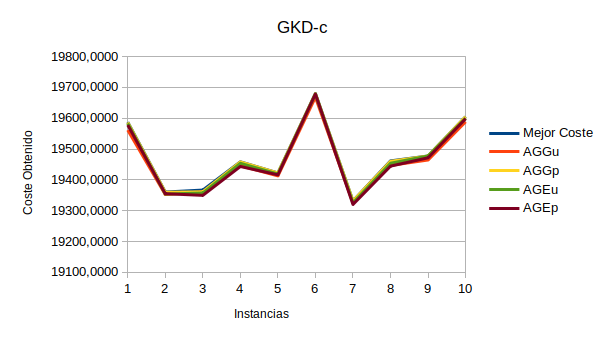
\includegraphics[scale=0.55]{img/gkdc.png}
	\end{figure}
	
	
	
	
	\item \texttt{MDG-a}: Conjunto de datos correspondiente al grupo de distancias enteras y tamaño de $n=2000$ y $m=200$. 
	
		
	\begin{figure}[H]
		\centering
		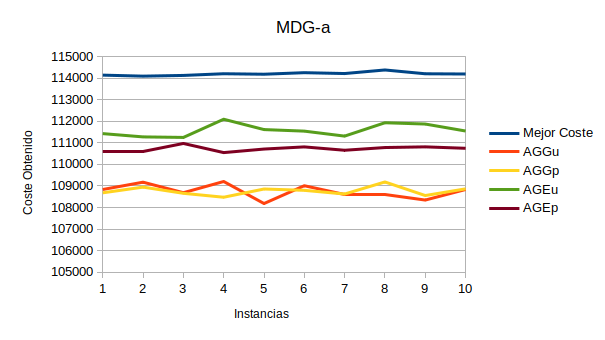
\includegraphics[scale=0.55]{img/mdga.png}
	\end{figure}
	
	En todas las muestras los costes obtenidos en el  AGE se encuentra sobre AGG, en sus dos variantes. En el AGE se aprecia que el que usa cruce uniforme tiene una mayor convergencia y esto es debido a que el cruce posicional es más disruptivo y comparte menos información de los padres. Esto no ocurre en el caso del AGG, donde se ve que no hay un claro ganador.
	
	
	

	
	
	
	\item \texttt{MDG-b}: Conjunto de datos correspondiente al grupo de distancias reales y tamaño $n=500$ y $m=50$. 
	
	
		
	\begin{figure}[H]
		\centering
		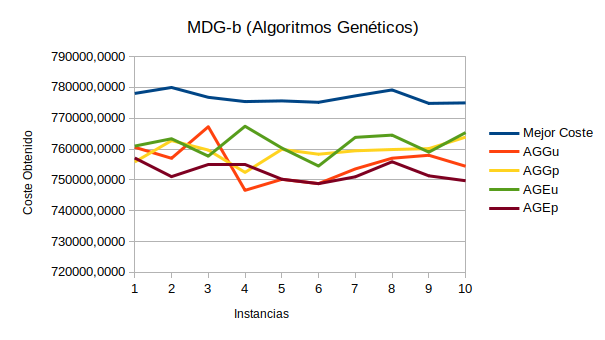
\includegraphics[scale=0.6]{img/mdgb.png}
	\end{figure}
	
	Se puede ver que la línea verde mayoritariamente está por encima del resto, es decir,
	al igual que en el caso anterior, el algoritmo de AGE con la estrategia de cruce uniforme mejora los costes de los otros algoritmos. Sin embargo, lo que se gana en eficacia se pierde en eficiencia, ya que si observamos la tabla de resultados globales \ref{glob}, el AGEu es el que tiene un mayor tiempo de ejecución de media, en total 315,41 segundos (Casi duplicando el resto de tiempos de los AG).
	
	
	Por otro lado y en segundo lugar se encuentra el AGG con cruce posicional que mejora respecto a su variante de cruce uniforme y será entonces el elegido para la implementación de los Algoritmos Meméticos.
	
	
	

	
\end{itemize}




\newpage 
\subsection{Algorítmos Meméticos}

Como hemos comentado en el punto anterior, el AGG que se ha usado para la población ha sido el del cruce basado en posición, aunque por muy pocas décimas. \ref{glob}. Los resultados en general han sido muy satisfactorios, mejorando como era de esperar los resultados de BL y AGG por separado.


La hibridación de los Algoritmos Meméticos no solo ha mejorado en eficacia sino que su eficiencia también se ha visto favorecida. Ésta ha aumentado, obteniendo un tiempo de ejecución bastante inferior respecto al AGG original, coincidiendo con el caso teórico esperado. Esto es debido a que la BL implementada en la práctica 1 realizaba una factorización de la función objetivo, no siendo necesario recalcular el coste de ls solución obtenida (bastaba con sumar y restar la contribución del elemento añadido y quitado, respectivamente). 



Mostramos para cada grupo \texttt{(GKD-c, MDG-a y MDG-b)} el coste obtenido para cada una de sus instancias:


\begin{figure}[H]
	\centering
	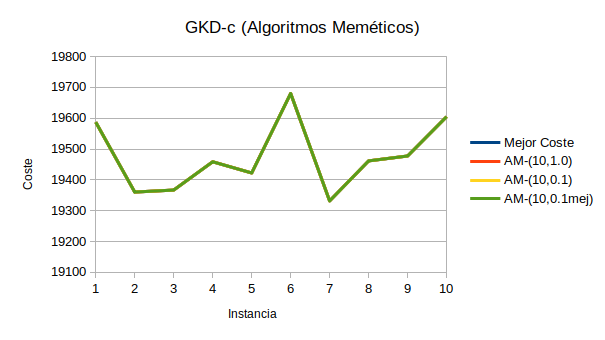
\includegraphics[scale=0.6]{img/amc.png}
\end{figure}

\begin{figure}[H]
	\centering
	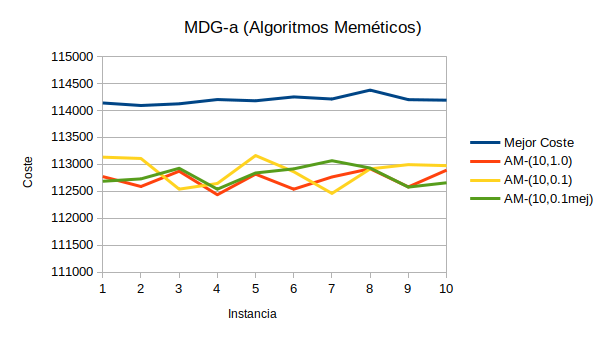
\includegraphics[scale=0.6]{img/ama.png}
\end{figure}

\begin{figure}[H]
	\centering
	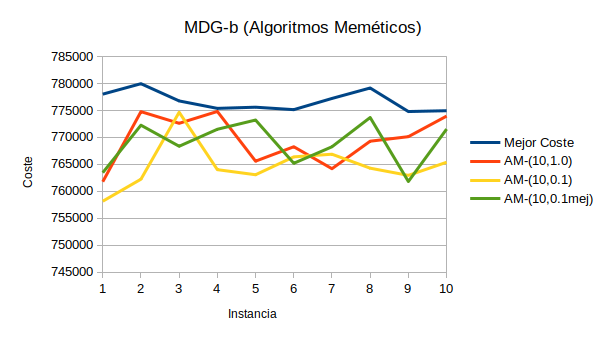
\includegraphics[scale=0.6]{img/amb.png}
\end{figure}



A simple vista, observando las gráficas anteriores, no hay un claro vencedor. Sin embargo, en la gráfica de \texttt{MDG-b}, la línea amarilla referente a \texttt{AM-(10,0.1)} se encuentra mayoritariamente por debajo del resto lo que se ve reflejado en una leve peor desviación en la tabla \ref{glob}.

Si recordamos esta variante, consistía en aplicar BL a un determinado número de cromosomas elegidos de forma aleatoria. Como era de esperar, la aleatoriedad no se lleva bien (en este caso) con los algoritmos y, de hecho, los mejores resultados se obtienen en \texttt{AM-(10,1.0)} y \texttt{AM-(10,0.1mej)} donde no hay un factor aleatorio sino que se aplica la BL sobre todos los cromosomas y sobre los mejores cromosomas, respectivamente.



\newpage 
\subsection{Desviación y tiempo}
Por último, reflejamos en un par de gráficos la desviación y el tiempo obtenidos de media para cada uno de los algoritmos implementados tanto en la práctica 1 como en la 2.

Conviene destacar que los algoritmos que peores resultados arrojan son los Algoritmos Genéticos Generacionales, obteniendo una desviación incluso peor que el algoritmo Greedy. Como norma general, el Greedy suele ser uno de los algoritmos que peor se adapta en cuanto a resultados al problema, sin embargo, en nuestro caso no es así.





\begin{figure}[H]
	\centering
	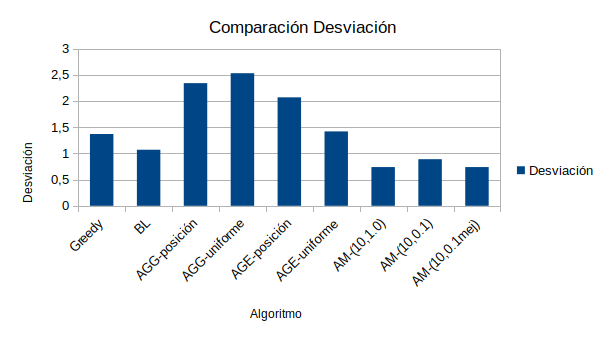
\includegraphics[scale=0.6]{img/res1.png}
	
\end{figure}


En lo referente al tiempo, los algoritmos genéticos se llevan la derrota. Como se ha comentado anteriormente, la mejor variante en coste ha sido AGEu, pero también ha sido la peor en tiempo.

Por otro lado, la técnica BL tanto individual como en sus versiones hibridadas de los Algoritmos Meméticos en nuestro problema MDP ha sido un gran logro tanto en eficacia como en eficiencia obteniendo unos resultados casi óptimos y ejecutando casi todas las instancias por debajo de los 50 segundos.

\begin{figure}[H]
	\centering
	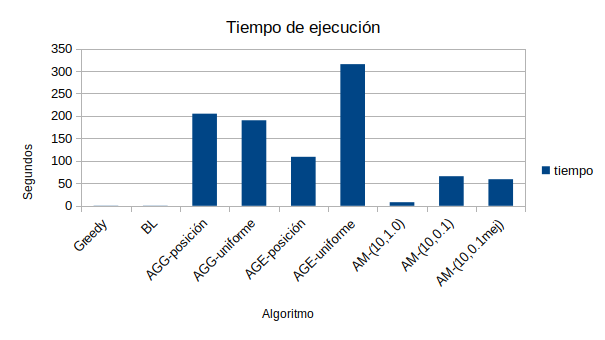
\includegraphics[scale=0.6]{img/time.png}
	
\end{figure}






\newpage

\section{Ejercicio extra}

Durante la realización de esta práctica me ha parecido muy interesante el equilibrio entre exploración y explotación llevado a cabo en las variantes de nuestro algoritmo memético y cómo aumentando un enfoque u otro se pueden obtener unos mejores resultados. \\



Recordando la sección 5, la variante \texttt{AM-(10,1.0)} aplicaba BL sobre todos los cromosomas, \texttt{AM-(10,0.1)} aplicaba BL a un subconjunto de cromosomas de la población elegido de forma aleatoria y \texttt{AM-(10,0.1mej)} aplicaba BL sobre los \textbf{0.1$\cdot$mejores} cromosomas de la población actual. El problema de estos casos es que la exploración era algo débil ya que la BL consumía todas las evaluaciones de la función objetivo. Por ello, establecemos un nuevo criterio de parada de 600 generaciones (en torno al doble) para olvidarnos del problema de la exploración y  así establecer una heurística de explotación para obtener un resultado óptimo para nuestro problema MDP. \\

Para ello, se han programado tres nuevas variantes:



\begin{itemize}
	\item \texttt{AM-(greedy1)}: Es el Algoritmo Memético en su versión más greedy. A la hora de aplicar BL, se explora el cromosoma que mejor coste tiene de toda la población, es decir, se elige la opción óptima en cada paso local, con la esperanza de llegar a una solución general óptima. 
	
	
	Nos podemos encontrar situaciones en las que uno de los cromosomas sea bueno en comparación con el resto de cromosomas de la población pero no lo sea tanto para el problema MDP. Si este cromosoma se encuentra en un óptimo local, se aplicará BL sobre éste pero no saldrá de este óptimo, obstaculizando así la exploración del resto de cromosomas.

	
	
	\item \texttt{AM-(greedy2)}: Versión greedy en la que se intentan evitar óptimos locales. En vez de explorar los cromosomas que más coste tienen, se exploran los que menos. Con esto, se evitarán más óptimos locales ya que se explora un abanico más grande de cromosomas.
	Sin embargo, nos encontramos en el dilema de estar explorando cromosomas no prometedores para evitar óptimos locales.
	
	\item \texttt{AM-(worst)}: Para la implementación de esta versión me he basado en la idea del operador de reparación del operador de cruce Uniforme usado en nuestros Algoritmos Genéticos y propuesto en el Seminario 3. Cuando corresponda, se aplica BL sobre el subconjunto de $n/2$ \textbf{peores} cromosomas (donde n es el tamaño de la población). Con esto, ganamos diversidad ya que exploramos también las soluciones menos prometedoras y, además, el problema de los óptimos locales deja de serlo ya que el subconjunto donde se aplica BL es suficientemente grande.
	
\end{itemize}








\newpage

Mostramos a continuación el pseudocódigo de las tres versiones:




\begin{figure}[H]
	\centering
	\begin{minipage}{.9\linewidth}
		
		
		
		\begin{algorithm}[H] 
			
			\caption{Algoritmos Meméticos}
			\SetAlgoLined
			
			\KwData{\textbf{Algoritmos Meméticos}}
			
			\Begin{
				
				
				\hfill \break 
				\text{ } \textbf{case} \texttt{ AM-(greedy1):} \break 
				\text{  } \hspace{0.3cm} $n\_mejores \leftarrow prob\_ls \cdot n$ \;
				\text{  } \hspace{0.5cm} \textbf{mientras} $n\_mejores>0$ \{ \break
				\text{  } \hspace{0.8cm} $i \leftarrow best\_element(poblacion)$ \;
				\text{  } \hspace{1cm} $cromosoma \leftarrow poblacion[i]$ \;
				\text{  } \hspace{1cm} $poblacion[i]$ $\leftarrow$ \textbf{BusquedaLocal}\textit{(cromosoma , eval)}\;
				\text{  } \hspace{1cm} \textit{n\_mejores - -} \;
				\text{  } \hspace{0.5cm} \} \break
				\text{} \hspace{0.4cm} \textbf{break} \;
				
				
				
								
				\hfill \break 
\text{ } \textbf{case} \texttt{ AM-(greedy1):} \break 
\text{  } \hspace{0.3cm} $n\_peores \leftarrow prob\_ls \cdot n$ \;
\text{  } \hspace{0.5cm} \textbf{mientras} $n\_peores>0$ \{ \break
\text{  } \hspace{0.8cm} $i \leftarrow worst\_element(poblacion)$ \;
\text{  } \hspace{1cm} $cromosoma \leftarrow poblacion[i]$ \;
\text{  } \hspace{1cm} $poblacion[i]$ $\leftarrow$ \textbf{BusquedaLocal}\textit{(cromosoma , eval)}\;
\text{  } \hspace{1cm} \textit{n\_peores - -} \;
\text{  } \hspace{0.5cm} \} \break
\text{} \hspace{0.4cm} \textbf{break} \;
				
				
				
				
				\hfill \break 
				\text{ } \textbf{case} \texttt{ AM-(worst):} \break 
				\text{  } \hspace{0.3cm} $n\_peores \leftarrow n/2$ \;
				\text{  } \hspace{0.5cm} $aux \leftarrow$ \textit{Índices de los n\_peores cromosomas}\; \break
				\text{  } \hspace{0.5cm} \textbf{para} \textit{i in $aux$} \textbf{hacer}\{ \break
				\text{  } \hspace{0.8cm} $cromosoma$ $\leftarrow$ $poblacion[i]$ \;
				\text{  } \hspace{1cm} $poblacion[i]$ $\leftarrow$ \textbf{BusquedaLocal}\textit{($cromosoma$ , eval)}\;
				\text{  } \hspace{0.5cm} \} \break
				\text{} \hspace{0.4cm} \textbf{break} \;

				
				
			}
			
		\end{algorithm} 
		
	\end{minipage}
\end{figure}



\newpage

\subsection{Resultados}



% Please add the following required packages to your document preamble:
% \usepackage{booktabs}
% \usepackage{graphicx}
% \usepackage[table,xcdraw]{xcolor}
% If you use beamer only pass "xcolor=table" option, i.e. \documentclass[xcolor=table]{beamer}
\begin{table}[H]
	\centering
	\resizebox{\textwidth}{!}{%
		\begin{tabular}{@{}
				>{\columncolor[HTML]{FFFFFF}}c 
				>{\columncolor[HTML]{FFFFFF}}c 
				>{\columncolor[HTML]{FFFFFF}}c 
				>{\columncolor[HTML]{FFFFFF}}c 
				>{\columncolor[HTML]{FFFFFF}}c 
				>{\columncolor[HTML]{FFFFFF}}c 
				>{\columncolor[HTML]{FFFFFF}}c 
				>{\columncolor[HTML]{FFFFFF}}c @{}}
			\toprule
			{\color[HTML]{333333} \textbf{Instancia}}     & {\color[HTML]{333333} \textbf{Mejor Coste}} & {\color[HTML]{333333} \textbf{AM-Greedy1}} & {\color[HTML]{333333} \textbf{Desv}} & {\color[HTML]{333333} \textbf{AM-Greedy2}} & {\color[HTML]{333333} \textbf{Desv}} & {\color[HTML]{333333} \textbf{AM-Worst}} & {\color[HTML]{333333} \textbf{Desv}} \\ \midrule
			{\color[HTML]{333333} GKD-c\_11\_n500\_m50}   & {\color[HTML]{333333} 19587,13}             & {\color[HTML]{333333} 19587,1}             & {\color[HTML]{333333} 0,00}          & {\color[HTML]{333333} 19587,1}             & {\color[HTML]{333333} 0,00}          & {\color[HTML]{333333} 19587,1}           & {\color[HTML]{333333} 0,00}          \\
			{\color[HTML]{333333} GKD-c\_12\_n500\_m50}   & {\color[HTML]{333333} 19360,24}             & {\color[HTML]{333333} 19360,2}             & {\color[HTML]{333333} 0,00}          & {\color[HTML]{333333} 19360,2}             & {\color[HTML]{333333} 0,00}          & {\color[HTML]{333333} 19360,2}           & {\color[HTML]{333333} 0,00}          \\
			{\color[HTML]{333333} GKD-c\_13\_n500\_m50}   & {\color[HTML]{333333} 19366,70}             & {\color[HTML]{333333} 19366,7}             & {\color[HTML]{333333} 0,00}          & {\color[HTML]{333333} 19366,7}             & {\color[HTML]{333333} 0,00}          & {\color[HTML]{333333} 19366,7}           & {\color[HTML]{333333} 0,00}          \\
			{\color[HTML]{333333} GKD-c\_14\_n500\_m50}   & {\color[HTML]{333333} 19458,56}             & {\color[HTML]{333333} 19458,6}             & {\color[HTML]{333333} 0,00}          & {\color[HTML]{333333} 19458,6}             & {\color[HTML]{333333} 0,00}          & {\color[HTML]{333333} 19458,6}           & {\color[HTML]{333333} 0,00}          \\
			{\color[HTML]{333333} GKD-c\_15\_n500\_m50}   & {\color[HTML]{333333} 19422,15}             & {\color[HTML]{333333} 19422,1}             & {\color[HTML]{333333} 0,00}          & {\color[HTML]{333333} 19422,1}             & {\color[HTML]{333333} 0,00}          & {\color[HTML]{333333} 19422,1}           & {\color[HTML]{333333} 0,00}          \\
			{\color[HTML]{333333} GKD-c\_16\_n500\_m50}   & {\color[HTML]{333333} 19680,21}             & {\color[HTML]{333333} 19680,2}             & {\color[HTML]{333333} 0,00}          & {\color[HTML]{333333} 19680,2}             & {\color[HTML]{333333} 0,00}          & {\color[HTML]{333333} 19680,2}           & {\color[HTML]{333333} 0,00}          \\
			{\color[HTML]{333333} GKD-c\_17\_n500\_m50}   & {\color[HTML]{333333} 19331,39}             & {\color[HTML]{333333} 19331,4}             & {\color[HTML]{333333} 0,00}          & {\color[HTML]{333333} 19328,4}             & {\color[HTML]{333333} 0,02}          & {\color[HTML]{333333} 19331,4}           & {\color[HTML]{333333} 0,00}          \\
			{\color[HTML]{333333} GKD-c\_18\_n500\_m50}   & {\color[HTML]{333333} 19461,39}             & {\color[HTML]{333333} 19461,4}             & {\color[HTML]{333333} 0,00}          & {\color[HTML]{333333} 19461,4}             & {\color[HTML]{333333} 0,00}          & {\color[HTML]{333333} 19461,4}           & {\color[HTML]{333333} 0,00}          \\
			{\color[HTML]{333333} GKD-c\_19\_n500\_m50}   & {\color[HTML]{333333} 19477,39}             & {\color[HTML]{333333} 19477,3}             & {\color[HTML]{333333} 0,00}          & {\color[HTML]{333333} 19477,3}             & {\color[HTML]{333333} 0,00}          & {\color[HTML]{333333} 19477,3}           & {\color[HTML]{333333} 0,00}          \\
			{\color[HTML]{333333} GKD-c\_20\_n500\_m50}   & {\color[HTML]{333333} 19604,84}             & {\color[HTML]{333333} 19604,8}             & {\color[HTML]{333333} 0,00}          & {\color[HTML]{333333} 19604,8}             & {\color[HTML]{333333} 0,00}          & {\color[HTML]{333333} 19604,8}           & {\color[HTML]{333333} 0,00}          \\
			{\color[HTML]{333333} MDG-b\_1\_n500\_m50}    & {\color[HTML]{333333} 778030,62}            & {\color[HTML]{333333} 766611}              & {\color[HTML]{333333} 1,47}          & {\color[HTML]{333333} 767828}              & {\color[HTML]{333333} 1,31}          & {\color[HTML]{333333} 768717}            & {\color[HTML]{333333} 1,20}          \\
			{\color[HTML]{333333} MDG-b\_2\_n500\_m50}    & {\color[HTML]{333333} 779963,69}            & {\color[HTML]{333333} 762531}              & {\color[HTML]{333333} 2,24}          & {\color[HTML]{333333} 766806}              & {\color[HTML]{333333} 1,69}          & {\color[HTML]{333333} 764921}            & {\color[HTML]{333333} 1,93}          \\
			{\color[HTML]{333333} MDG-b\_3\_n500\_m50}    & {\color[HTML]{333333} 776768,44}            & {\color[HTML]{333333} 774819}              & {\color[HTML]{333333} 0,25}          & {\color[HTML]{333333} 770896}              & {\color[HTML]{333333} 0,76}          & {\color[HTML]{333333} 773699}            & {\color[HTML]{333333} 0,40}          \\
			{\color[HTML]{333333} MDG-b\_4\_n500\_m50}    & {\color[HTML]{333333} 775394,62}            & {\color[HTML]{333333} 767390}              & {\color[HTML]{333333} 1,03}          & {\color[HTML]{333333} 767084}              & {\color[HTML]{333333} 1,07}          & {\color[HTML]{333333} 770724}            & {\color[HTML]{333333} 0,60}          \\
			{\color[HTML]{333333} MDG-b\_5\_n500\_m50}    & {\color[HTML]{333333} 775611,06}            & {\color[HTML]{333333} 769639}              & {\color[HTML]{333333} 0,77}          & {\color[HTML]{333333} 767524}              & {\color[HTML]{333333} 1,04}          & {\color[HTML]{333333} 774024}            & {\color[HTML]{333333} 0,20}          \\
			{\color[HTML]{333333} MDG-b\_6\_n500\_m50}    & {\color[HTML]{333333} 775153,69}            & {\color[HTML]{333333} 768731}              & {\color[HTML]{333333} 0,83}          & {\color[HTML]{333333} 769179}              & {\color[HTML]{333333} 0,77}          & {\color[HTML]{333333} 768685}            & {\color[HTML]{333333} 0,83}          \\
			{\color[HTML]{333333} MDG-b\_7\_n500\_m50}    & {\color[HTML]{333333} 777232,87}            & {\color[HTML]{333333} 765342}              & {\color[HTML]{333333} 1,53}          & {\color[HTML]{333333} 766411}              & {\color[HTML]{333333} 1,39}          & {\color[HTML]{333333} 769942}            & {\color[HTML]{333333} 0,94}          \\
			{\color[HTML]{333333} MDG-b\_8\_n500\_m50}    & {\color[HTML]{333333} 779168,75}            & {\color[HTML]{333333} 762033}              & {\color[HTML]{333333} 2,20}          & {\color[HTML]{333333} 773812}              & {\color[HTML]{333333} 0,69}          & {\color[HTML]{333333} 772572}            & {\color[HTML]{333333} 0,85}          \\
			{\color[HTML]{333333} MDG-b\_9\_n500\_m50}    & {\color[HTML]{333333} 774802,19}            & {\color[HTML]{333333} 765032}              & {\color[HTML]{333333} 1,26}          & {\color[HTML]{333333} 768830}              & {\color[HTML]{333333} 0,77}          & {\color[HTML]{333333} 770562}            & {\color[HTML]{333333} 0,55}          \\
			{\color[HTML]{333333} MDG-b\_10\_n500\_m50}   & {\color[HTML]{333333} 774961,31}            & {\color[HTML]{333333} 764799}              & {\color[HTML]{333333} 1,31}          & {\color[HTML]{333333} 767798}              & {\color[HTML]{333333} 0,92}          & {\color[HTML]{333333} 766434}            & {\color[HTML]{333333} 1,10}          \\
			{\color[HTML]{333333} MDG-a\_31\_n2000\_m200} & {\color[HTML]{333333} 114139}               & {\color[HTML]{333333} 112746}              & {\color[HTML]{333333} 1,22}          & {\color[HTML]{333333} 111932}              & {\color[HTML]{333333} 1,93}          & {\color[HTML]{333333} 113334}            & {\color[HTML]{333333} 0,71}          \\
			{\color[HTML]{333333} MDG-a\_32\_n2000\_m200} & {\color[HTML]{333333} 114092}               & {\color[HTML]{333333} 112680}              & {\color[HTML]{333333} 1,24}          & {\color[HTML]{333333} 112054}              & {\color[HTML]{333333} 1,79}          & {\color[HTML]{333333} 113164}            & {\color[HTML]{333333} 0,81}          \\
			{\color[HTML]{333333} MDG-a\_33\_n2000\_m200} & {\color[HTML]{333333} 114124}               & {\color[HTML]{333333} 112586}              & {\color[HTML]{333333} 1,35}          & {\color[HTML]{333333} 112270}              & {\color[HTML]{333333} 1,62}          & {\color[HTML]{333333} 113120}            & {\color[HTML]{333333} 0,88}          \\
			{\color[HTML]{333333} MDG-a\_34\_n2000\_m200} & {\color[HTML]{333333} 114203}               & {\color[HTML]{333333} 112502}              & {\color[HTML]{333333} 1,49}          & {\color[HTML]{333333} 112032}              & {\color[HTML]{333333} 1,90}          & {\color[HTML]{333333} 113508}            & {\color[HTML]{333333} 0,61}          \\
			{\color[HTML]{333333} MDG-a\_35\_n2000\_m200} & {\color[HTML]{333333} 114180}               & {\color[HTML]{333333} 112790}              & {\color[HTML]{333333} 1,22}          & {\color[HTML]{333333} 112053}              & {\color[HTML]{333333} 1,86}          & {\color[HTML]{333333} 113439}            & {\color[HTML]{333333} 0,65}          \\
			{\color[HTML]{333333} MDG-a\_36\_n2000\_m200} & {\color[HTML]{333333} 114252}               & {\color[HTML]{333333} 112698}              & {\color[HTML]{333333} 1,36}          & {\color[HTML]{333333} 112148}              & {\color[HTML]{333333} 1,84}          & {\color[HTML]{333333} 113189}            & {\color[HTML]{333333} 0,93}          \\
			{\color[HTML]{333333} MDG-a\_37\_n2000\_m200} & {\color[HTML]{333333} 114213}               & {\color[HTML]{333333} 112615}              & {\color[HTML]{333333} 1,40}          & {\color[HTML]{333333} 112142}              & {\color[HTML]{333333} 1,81}          & {\color[HTML]{333333} 113205}            & {\color[HTML]{333333} 0,88}          \\
			{\color[HTML]{333333} MDG-a\_38\_n2000\_m200} & {\color[HTML]{333333} 114378}               & {\color[HTML]{333333} 112851}              & {\color[HTML]{333333} 1,34}          & {\color[HTML]{333333} 112452}              & {\color[HTML]{333333} 1,68}          & {\color[HTML]{333333} 113462}            & {\color[HTML]{333333} 0,80}          \\
			{\color[HTML]{333333} MDG-a\_39\_n2000\_m200} & {\color[HTML]{333333} 114201}               & {\color[HTML]{333333} 112348}              & {\color[HTML]{333333} 1,62}          & {\color[HTML]{333333} 112012}              & {\color[HTML]{333333} 1,92}          & {\color[HTML]{333333} 113091}            & {\color[HTML]{333333} 0,97}          \\
			{\color[HTML]{333333} MDG-a\_40\_n2000\_m200} & {\color[HTML]{333333} 114191}               & {\color[HTML]{333333} 112931}              & {\color[HTML]{333333} 1,10}          & {\color[HTML]{333333} 112477}              & {\color[HTML]{333333} 1,50}          & {\color[HTML]{333333} 113479}            & {\color[HTML]{333333} 0,62}          \\ \bottomrule
		\end{tabular}%
	}
	\caption{Resultados AM-Extra}
	\label{AMall}
\end{table}






\[
\begin{array}{r|*{4}{r}}{Algoritmo}&Desv&Tiempo\\\hline

{}AM-(10,1.0)&0,74&8,05\\

{}AM-(10,0.1)&0,89&65,92\\

{}AM-(10,0.1mej)&0,74&59,24\\

{}AM-(Greedy1)&0,87&19,48\\

{}AM-(Greedy2)&0,94&19,95\\

{}AM-(Worst)&0,55&19,71
\end{array}
\label{glob}
\]





\newpage
Como era de esperar por lo comentado anteriormente, tanto la versión \texttt{Greedy1} como \texttt{Greedy2} no mejoran respecto a las versiones implementadas (a pesar de tener un criterio de parada menos restrictivo). Por otro lado, el mejor algoritmo implementado hasta ahora ha sido \texttt{AM-(Worst)}, con un total de 0.55 de desviación media total y con un tiempo de ejecución relativamente bajo, 19,71 segundos de media.



	
\begin{figure}[H]
	\centering
	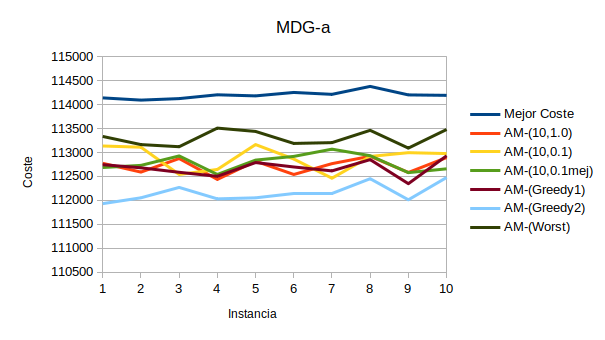
\includegraphics[scale=0.57]{img/gre.png}
\end{figure}



En las instancias de \texttt{GKD-c} todos los algoritmos llegan al óptimo global y en las de \texttt{MDG-b} se producen demasiados solapamientos y no permiten diferenciar muy bien los colores referentes a cada algoritmo. Sin embargo, en \texttt{MDG-a} la visualización es clara ya que nuestro problema MDP trabaja con una matriz de distancias de mayor tamaño. 





Como podemos observar, \texttt{AM-(Worst)} es el claro ganador en términos de convergencia y \texttt{AM-Greedy} en sus dos versiones implementadas son los peores. Esto nos deja como conclusión que no por una exploración más profunda se van a obtener mejores resultado sino que lo que realmente importa es la forma de hacerlo.




\newpage
\begin{thebibliography}{X} 
	
-\href{https://sci2s.ugr.es/sites/default/files/files/Teaching/GraduatesCourses/Metaheuristicas/Sem01-Problemas-MHs-2019-20.pdf}{Seminario 1}\\
	
	-\href{https://sci2s.ugr.es/sites/default/files/files/Teaching/GraduatesCourses/Metaheuristicas/Sem02-Problemas-BusquedaLocal-MHs-19-20.pdf}{Seminario 2}\\
	
		-\href{https://sci2s.ugr.es/sites/default/files/Sem03-Problemas-Poblaciones-MHs-19-20.pdf}{Seminario 3}\\
	
	-\href{https://sci2s.ugr.es/sites/default/files/files/Teaching/GraduatesCourses/Metaheuristicas/Guion\%20P1a\%20LocalGreedy\%20MDP\%20MHs\%202019-20.pdf}{Guión de prácticas}




\end{thebibliography}


\end{document}

